\documentclass[11pt]{amsart}
\usepackage{geometry} % see geometry.pdf on how tolay out the page. There's lots.
\usepackage{caption}
\usepackage{subcaption}
\usepackage{siunitx}
\usepackage{fancyhdr}
\usepackage{multicol}
\usepackage{graphicx}
\usepackage{amssymb}
\usepackage{amsmath}
\usepackage{mathtools}
\usepackage{booktabs}

\usepackage{pdflscape}
\usepackage[toc,page]{appendix}
\usepackage{float}
\usepackage{sidecap}
\usepackage{minted}
\usepackage{listings}
\usepackage{csquotes}


\usepackage[style=chicago-authordate]{biblatex} %Imports biblatex package
\usepackage{bm}
\usepackage{hyperref}

\DeclareMathOperator*{\argmax}{argmax}
\DeclareMathOperator*{\argmin}{argmin}

\geometry{a4paper} % orletter or a5paper or ... etc %
\geometry{left=2.5cm, right=2.5cm, bottom=2.5cm, top = 2.5cm}

\setlength{\intextsep}{5pt} % Vertical space above & below [h] floats
\setlength{\textfloatsep}{5pt} % Vertical space below (above) [t] ([b]) floats
\setlength{\abovecaptionskip}{3pt}
\setlength{\belowcaptionskip}{3pt}


\newenvironment{Figure}
  {\par\medskip\noindent\minipage{\linewidth}}
  {\endminipage\par\medskip}


\author{CCN: 5654F}
\title[4F13 - Coursework \#3: Latent Dirichlet Allocation]{\vspace*{-1.0cm}4F13 - Coursework \#3: Latent Dirichlet Allocation\vspace*{-0.5cm}}
\date{Wednesday 15th November 2023} % delete this line to display the current date4340-


%%% BEGIN DOCUMENT
\begin{document}
\maketitle
\vspace*{-1cm}
\section{Task A: Multinomial Maximum Likelihood} \label{sec:a}
The maximum likelihood multinomial assumes each word is drawn from one categorical distribution: $w_{nd} \sim \mathrm{Cat}\left(\bm{\beta}\right)$, where $\bm{\beta}$ is a vector containing the probability each word will be used. The maximum likelihood (ML) estimate for $\bm{\beta}$ for training set $\mathcal{A}$ is simply the empirical word frequency for each word, as seen in Equation \ref{eqn:beta_ml}, where $\bm{c}$ is the vector of counts of distinct word occurences in the document set. $\bm{c}$ is calculated as shown in Listing \ref{lst:cw3a}, and then divided by the total word count over the document, giving us $\hat{\bm{\beta}}_{ML}$.

\vspace{-0.4cm}
\small
\begin{equation} \label{eqn:beta_ml}
    \begin{aligned}
        \hat{\bm{\beta}}_{ML} & = \argmax_{\beta}\log\prod_{d=1}^{D}\prod_{n}^{N_d}\mathrm{Cat}\left(w_{nd}\vert\beta\right)  \\
                              & = \argmax_{\beta}\log\mathrm{Mult}\left(c_1,\dots,c_M\vert\beta, N\right)  = \frac{\bm{c}}{N} \\
    \end{aligned}
\end{equation}
\normalsize

\begin{listing}[h]
    \begin{minted}[linenos,breaklines,fontsize=\footnotesize]{python3}
        word_counts = np.zeros(W, dtype=int)  
        for doc_num in range(D):
            doc__word_indices = np.where(A[:, 0] == doc_num + 1)
            word_indices = np.array(A[doc_word_indices, 1])
            word_counts[word_indices - 1] += np.array(A[doc__word_indices, 2])
    \end{minted}
    \caption{Task A code excerpts} \label{lst:cw3a}
\end{listing}

The most and least probable words are then plotted in two bar plots, as shown in Figure \ref{fig:taska_all}. The highest log probability possible is generated when the test set contains only the most probable word: ``bush''. For a test set $L$ words long this is a log probability of $\log{{}\hat{\bm{\beta}}_{ML,\max}}^{L} = L\log0.0141 \approx -4.3L$ (0.0141 is the probability of ``bush''). The lowest log probability occurs when any of the words in the test set did not appear in the training set, giving a probability of 0 and a log probability of $-\infty$. This is a very oversimplistic model as it cannot handle words that do not appear in the training set.
\begin{figure}[h]
    \centering
    \begin{subfigure}[b]{0.49\textwidth}
        \centering
        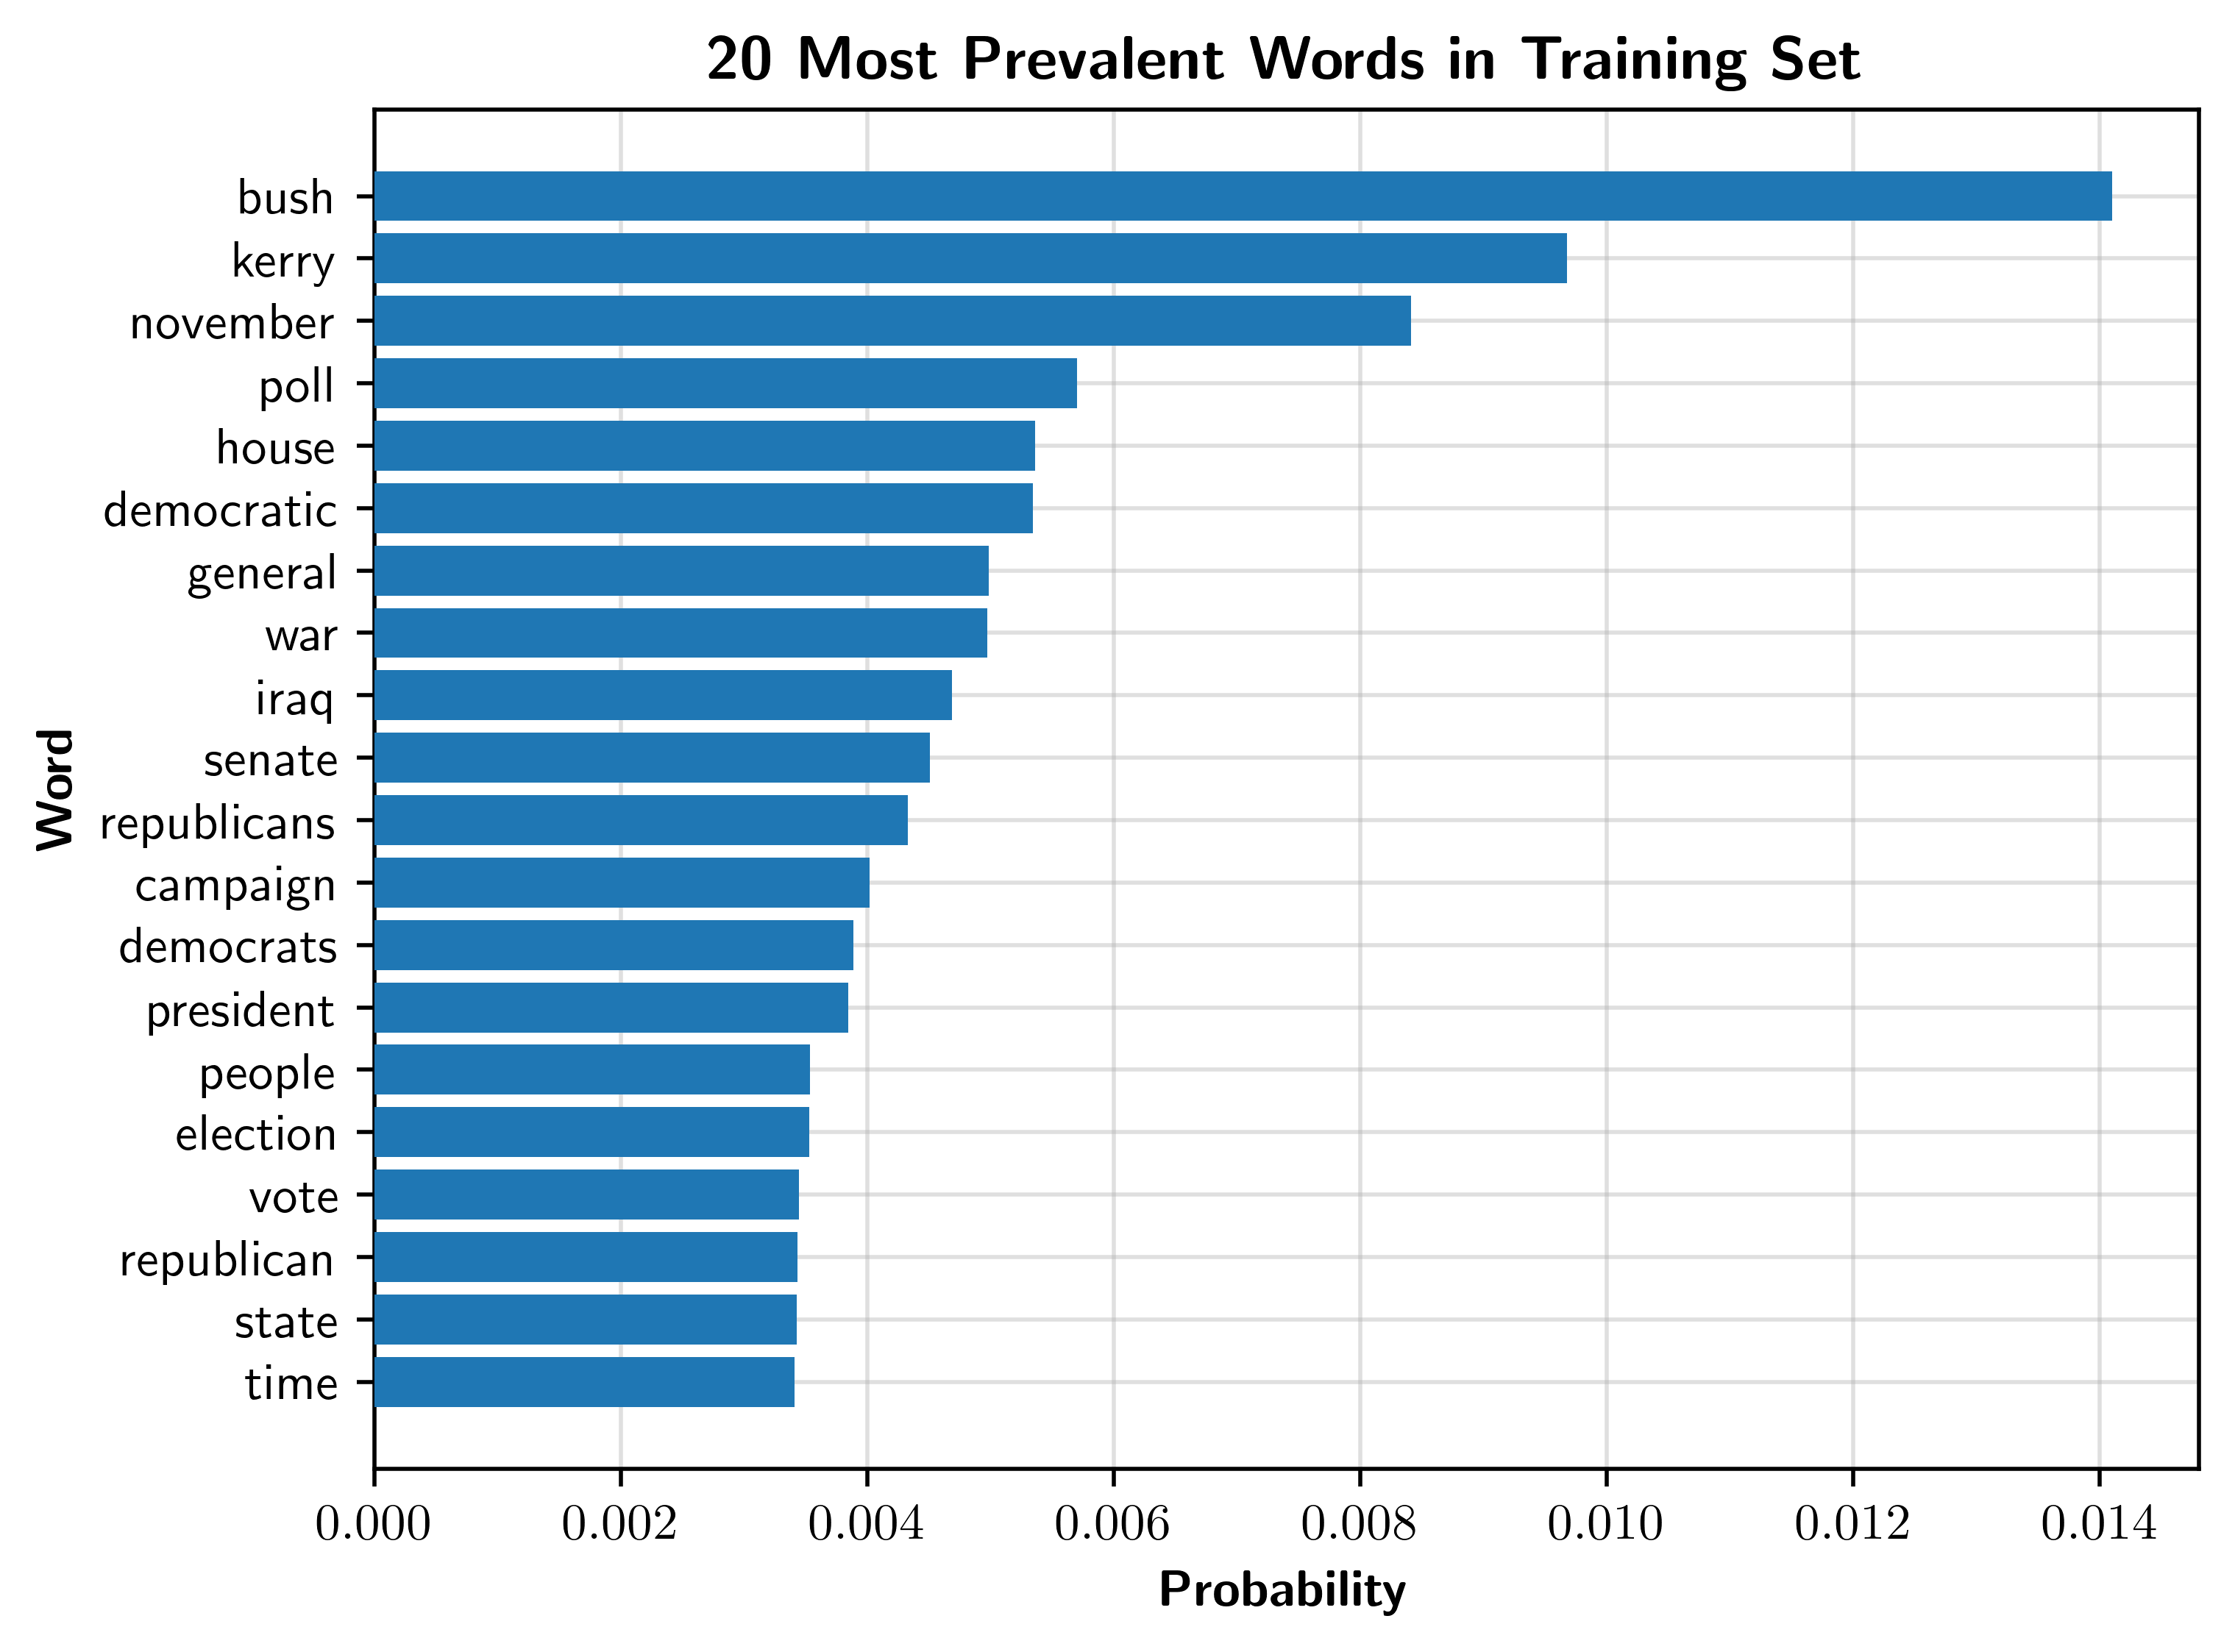
\includegraphics[width=0.99\textwidth]{../plots/a_histogram.png}
    \end{subfigure}
    \hfill
    \begin{subfigure}[b]{0.49\textwidth}
        \centering
        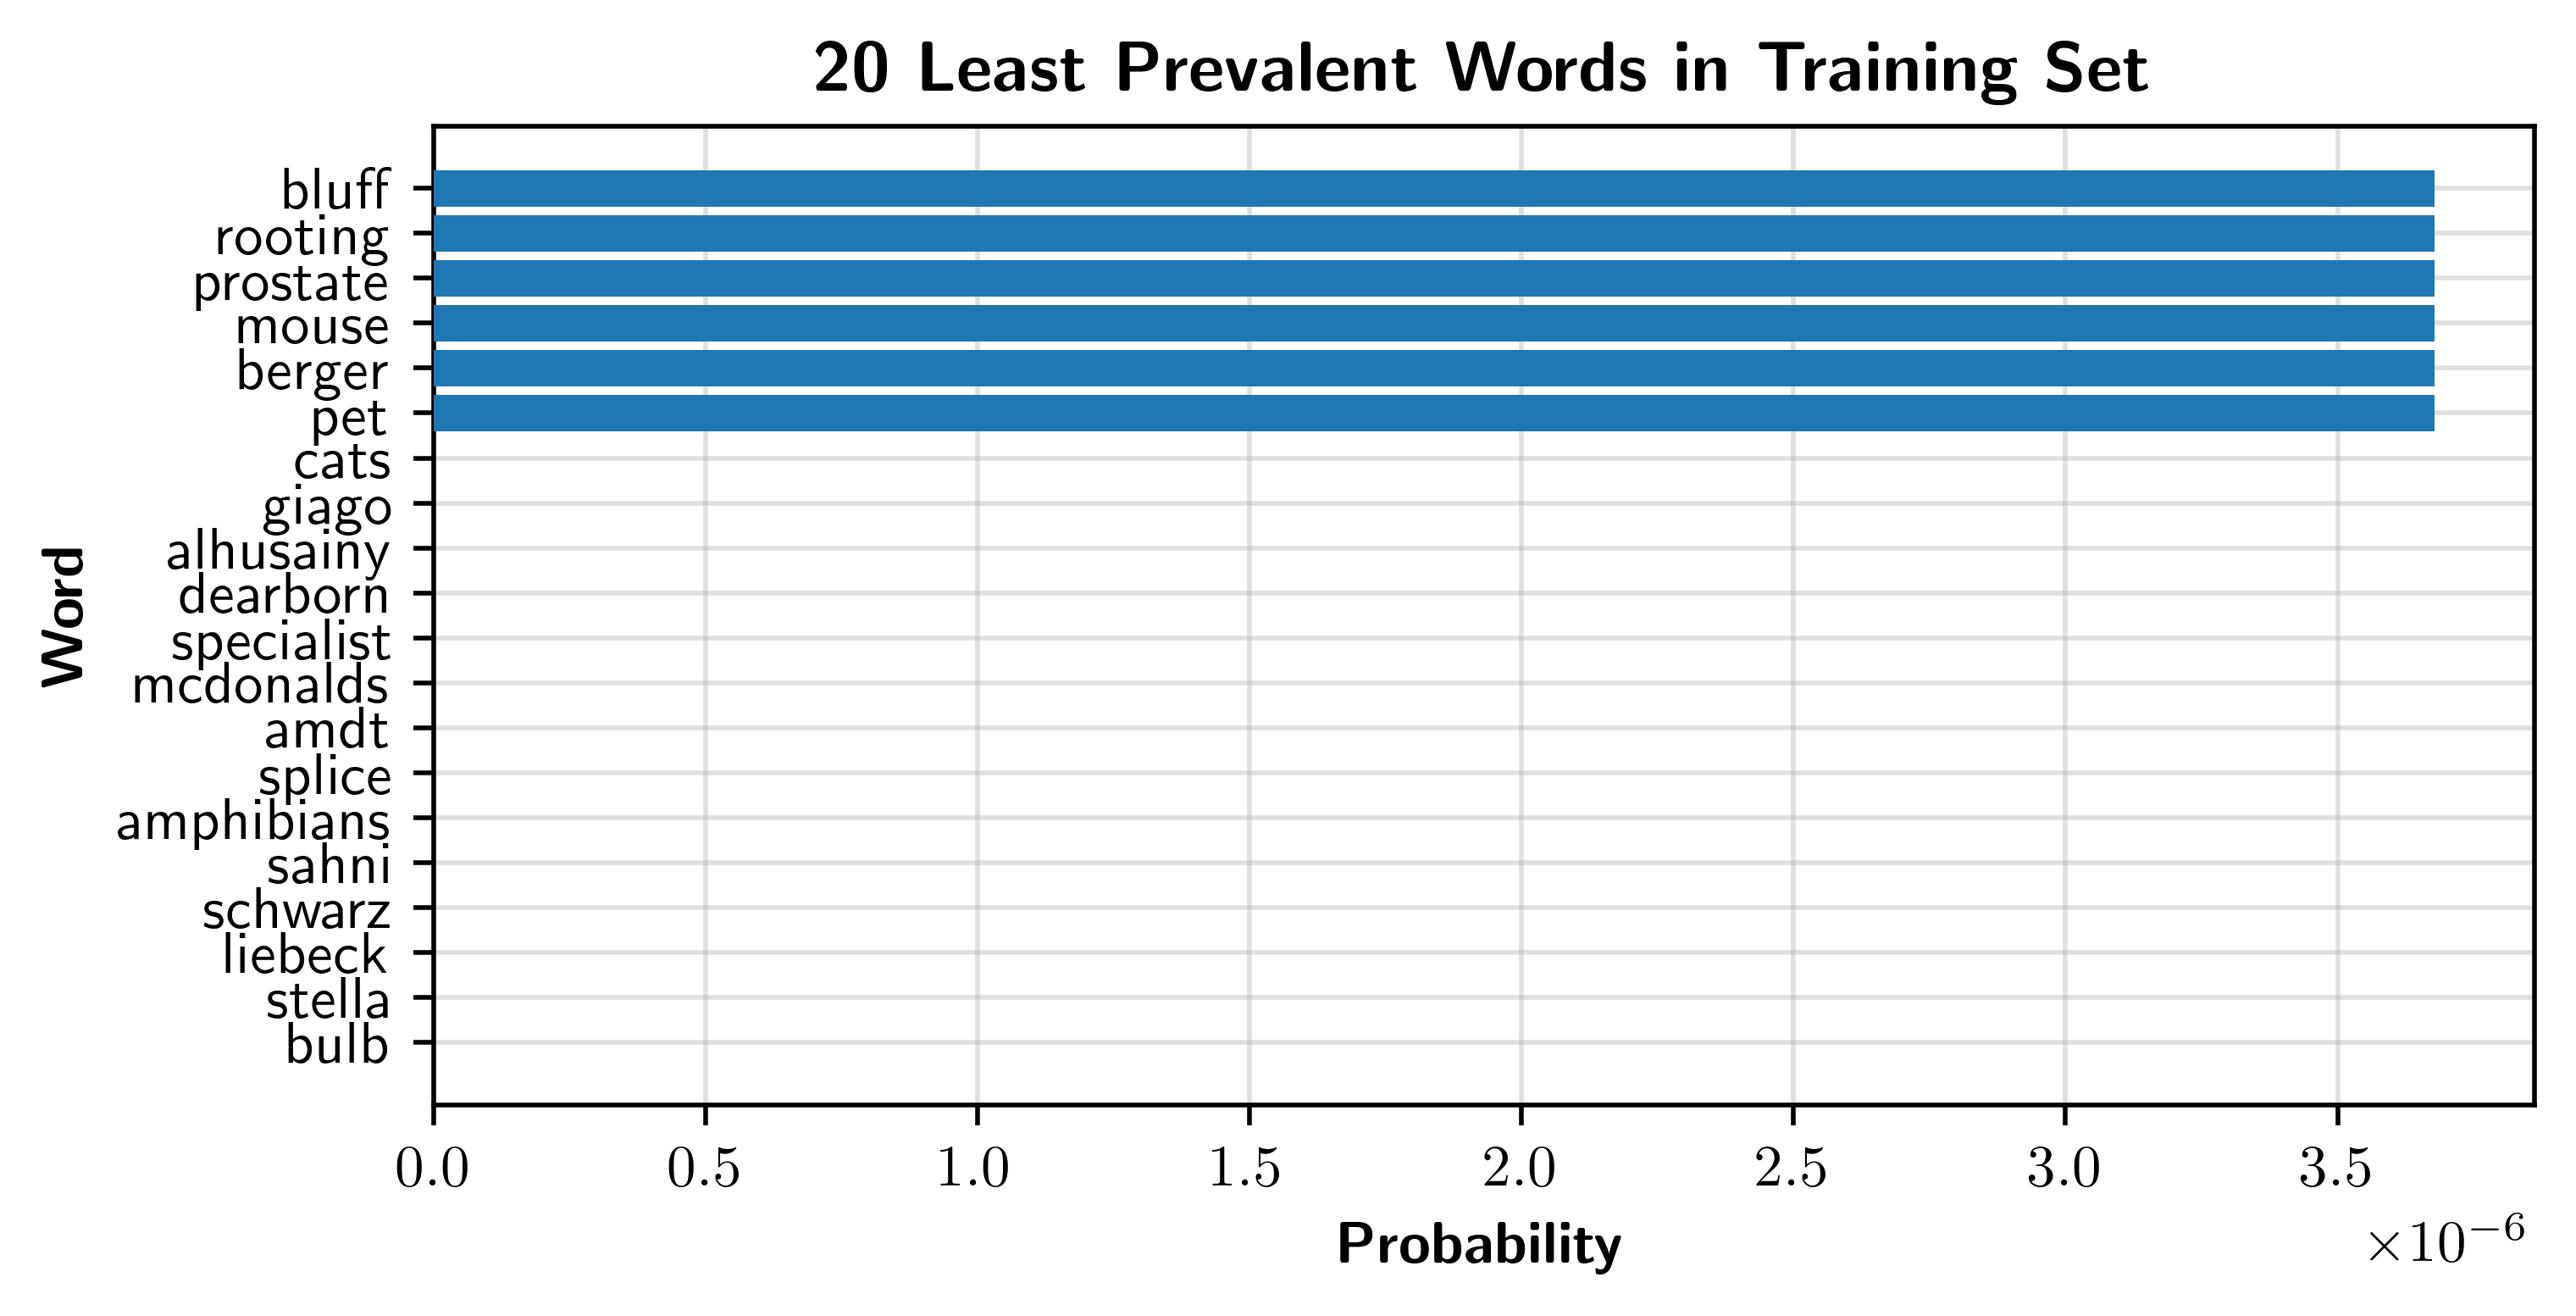
\includegraphics[width=0.99\textwidth]{../plots/a_histogram_bottom.png}
    \end{subfigure}
    \caption{Task A Figures}\label{fig:taska_all}
\end{figure}

\vspace*{-0.5cm}
\section{Task B: Dirichlet Prior} \label{sec:b}
The model was improved by adding a symmetric Dirichlet Prior: $\bm{\beta} \sim \mathrm{Dir}(\bm{\beta}, \alpha)$, with concentration parameter $\alpha$. Using Bayes Rule, the posterior distribution is calculated as in Equation \ref{eqn:b_posterior}, and as this is also a Dirichlet (due to the Dirichlet being a conjugate prior to the categorical), the maximum a posteriori (MAP) predictive distribution is as in Equation \ref{eqn:b_ml}. The effect of the prior is to add a pseudocount of $\alpha$ to each count, by adding the lines in Listing \ref{lst:cw3b}.

\vspace{-0.1cm}
\small
\begin{align}
    \begin{split} \label{eqn:b_posterior}
        P(\bm{\beta} \vert \mathcal{A}) & \propto  P(\bm{\beta}) \cdot P(\mathcal{A} \vert \bm{\beta}) \propto \prod_{m=1}^{M} {\beta_{M}}^{c_m}\prod_{m=1}^{M} {\beta_{M}}^{c_m+\alpha-1} \\
                                        & = \mathrm{Dir} (\bm{\beta}\vert \bm{c} + \alpha \cdot \mathbf{1})
    \end{split} \\
    \begin{split} \label{eqn:b_ml}
        \hat{\bm{\beta}}_{MAP} & = \frac{\bm{c} + \alpha\cdot\mathbf{1}}{\sum_{l=1}^{M}c_l + \alpha}
    \end{split}
\end{align}
\normalsize


\begin{listing}[h]
    \begin{minted}[linenos,breaklines,fontsize=\footnotesize]{python3}
        prior_counts = alpha * np.ones(W)
        posterior_counts = word_counts + prior_counts
        total_count = np.sum(posterior_counts)
    \end{minted}
    \caption{Task B code excerpts} \label{lst:cw3b}
\end{listing}

Figure \ref{fig:taskb} shows different posterior predictive distributions for different values of $\alpha$, for the top 20 and bottom 20 words (for $\alpha = 10$). The change is clear for the bottom 20 words: unseen words in training have a non-zero probability of occuring. As $\alpha$ increases the word probabilities become more uniform across the vocabulary. When $\alpha = 0$ the prior does nothing.
\begin{figure}[h]
    \centering
    \makebox[\textwidth]{
        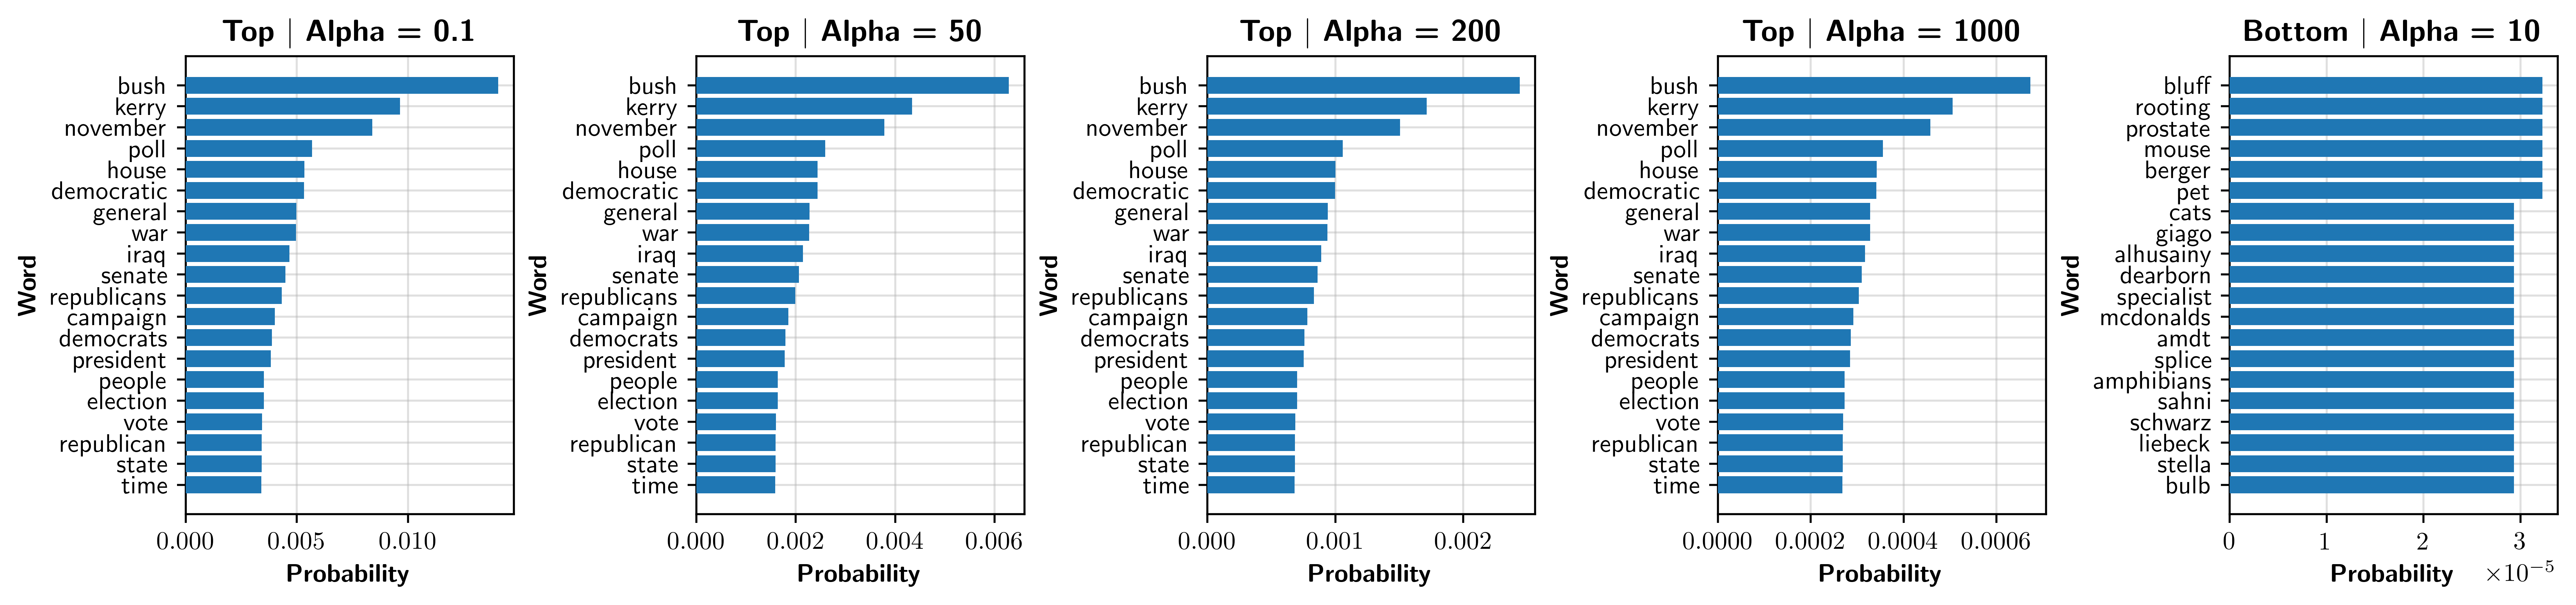
\includegraphics[width=1.1\textwidth]{../plots/b_pred_histogram_new.png}
    }
    \caption{Dirichlet Prior - Posterior Predictive Distributions} \label{fig:taskb}
\end{figure}

\vspace*{-0.5cm}
\section{Task C: Log Probabilities} \label{sec:c}
To calculate the log probability $L(d)$ of a test document $d$ using the Bayesian Model, Equation \ref{eqn:c_logp} is used. $\left\{w_{nd}^*\right\}^{N_d}_{n=1}$ is the set of words in $d$. $c_m^*$ is the count of word $m$ in $d$. The data we are given howvever is just the word counts for each document, not the word order, which is obviously an important part of document analysis. To account for this a combinatorial term could be added as in Equation \ref{eqn:c_comb}. However, we can consider all word orderings of documents to be equally likely for the moment and therefore this can be ignored and the categorical distribution function is used.

With $\alpha$ set to 0.1, the log probabiility of Document 2001 was calculated to be -3691.2, with 440 total words.

Also of use is the per-word perplexity, which is a measure of performance, and the definition is given in Equation \ref{eqn:c_pwpp}. Listing \ref{lst:cw3c} shows how the log probability and perplexity for Document 2001 were calculated.
\vspace{-0.1cm}
\small
\begin{align}
    \begin{split}  \label{eqn:c_logp}
        L\left(d\right) = \log P\left(\left\{w_{nd}^*\right\}^{N_d}_{n=1} \vert \mathcal{A}\right) & = \log\prod_{n=1}^{N_d}  P\left(w_{nd}^*\vert\mathcal{A}\right)  =  \sum_{n=1}^{N_d} \log P\left(w_{nd}^*\vert\mathcal{A}\right) \\& =\sum_{m=1}^{M} c_m^* \log P\left(w^* = m\vert\mathcal{A}\right)  = {\bm{c}^*}^T \log \hat{\bm{\beta}}^*
    \end{split} \\
    \begin{split} \label{eqn:c_comb}
        P\left(\left\{w_{nd}^*\right\}^{N_d}_{n=1} \vert \mathcal{A}\right) & = \frac{N_d!}{\prod_{m=1}^{M}c_m^*!}\prod_{n=1}^{N}P(w_{nd}^*\vert \hat{\bm{\beta}}^*)
    \end{split}                                                                                                                                                                       \\
    \begin{split} \label{eqn:c_pwpp}
        p(d) & = \exp\left(-\frac{L(d)}{N_d}\right)
    \end{split}
\end{align}
\normalsize

\begin{listing}[h]
    \begin{minted}[linenos,breaklines,fontsize=\footnotesize]{python3}
        log_posterior_frequencies = np.log(posterior_frequencies)
        test_doc_log_probability = np.dot(test_doc_word_counts, log_posterior_frequencies)
        test_doc_perplexity = np.exp(-1 * test_doc_log_probability / test_doc_total_words)
    \end{minted}
    \caption{Task C code excerpts} \label{lst:cw3c}
\end{listing}


\begin{table}[h]
    \centering{}
    \begin{center}
        \begin{tabular}{lccc}\toprule
            ---                 & Document 2001 & All Documents & Uniform Multinomial \\ \midrule
            Per-word Perplexity & \num{4399.0}  & \num{2697.1}  & \num{6906}          \\\bottomrule
        \end{tabular}%
        \par\end{center}
    \caption{Task C Perplexities} \label{tab:c_tab}

\end{table}

Table \ref{tab:c_tab} contains the per-word perplexities for Document 2001 of the test set $\mathcal{B}$ and the whole of $\mathcal{B}$, as well as the perplexity of $\mathcal{B}$ when using a uniform multinomial. This is just equal to the number of distinct words in $\mathcal{B}$, as a perplexity of $n$ implies a confidence the same as if an $n$-sided dice was choosing each word. Different documents have different perplexities due to the fact that they contain a different subset of the whole word set that is trained over. A document that has a higher proportion of words that were more common in the training set will have a higher log probability and therefore a lower (better) perplexity. Document 2001 has a much higher perplexity than $\mathcal{B}$ as a whole, and therefore must contain a higher proportion of words that are scarcer in $\mathcal{A}$ than the average.

% \vspace*{-0.75cm}
\section{Task D: Bayesian Mixture of Multinomials} \label{sec:d}
Figure \ref{fig:d_model} shows an overview of the model used in Task D. $z_d \in {1, \dots, K}$ is a latent variable denoting the topic of each document. The probability of a document being about topic $k$ is $\theta_k \in \bm{\theta}$, which is initialised with a symmetric Dirichlet prior.

The python function \verb|BMM| was provided which returns the test set perplexities and multinomial weights over words using gibbs sampling. The function was modified to return the number of documents assigned to each topic at each iteration by adding a new return array which contains a copy of \verb|sk_docs| at each iteration, as seen in Listing \ref{lst:cw3d}.

\begin{figure}[h]
    \centering
    \makebox[\textwidth]{
        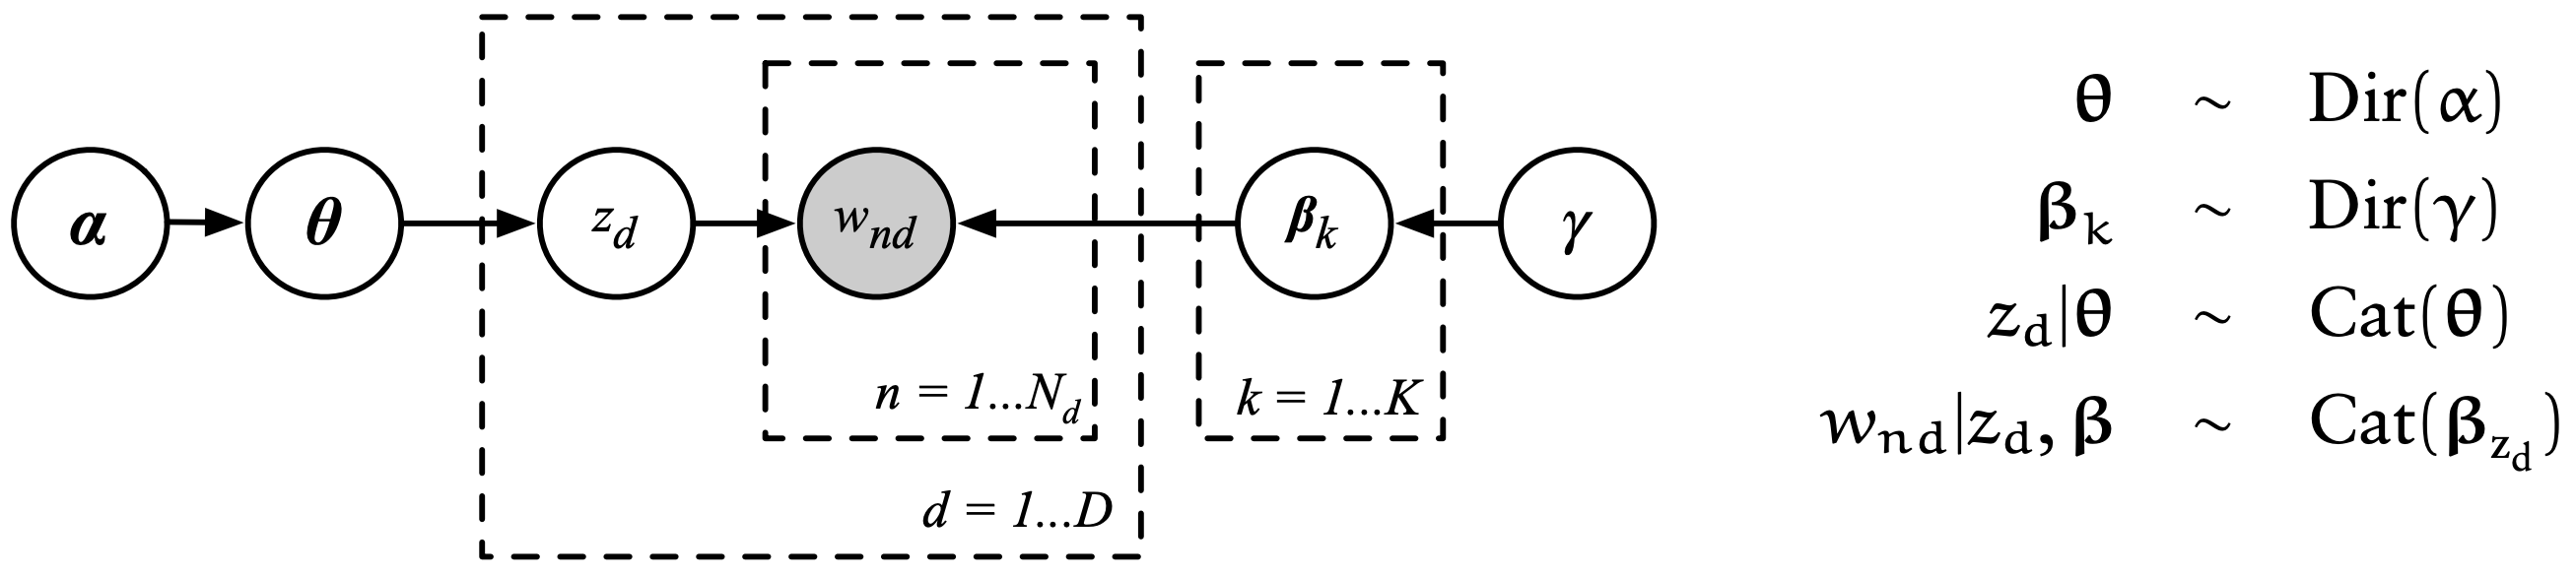
\includegraphics[width=0.7\textwidth]{../plots/Screenshot 2023-11-30 at 22.44.43.png}
    }
    \caption[Bayesian Mixture of Multinomials Model]{Bayesian Mixture of Multinomials Model\protect\footnotemark} \label{fig:d_model}
\end{figure}
\footnotetext{\label{fn:l_notes}CUED 4F13 Lecture notes \href{Uhttps://mlg.eng.cam.ac.uk/teaching/4f13/2324/RL}{(course site)}}


\begin{listing}[h]
    \begin{minted}[linenos,breaklines,fontsize=\footnotesize]{python3}
        sk_docs_history = np.zeros(
            (num_mixture_components, num_iters_gibbs + 1), dtype=int
        )
        sk_docs_history[:, 0] = np.copy(sk_docs)[:, 0]
        # ...
        for iteration in tqdm(range(num_iters_gibbs)):
            # Do gibbs ....
            sk_docs_history[:, iteration + 1] = np.copy(sk_docs)[:, 0]
    \end{minted}
    \caption{Task D code excerpts} \label{lst:cw3d}
\end{listing}

The model could then be trained using Gibbs Sampling over the training set using $\alpha = 10$ for the prior on mixture components and $\gamma = 0.1$ for the prior on words. The $\theta_k$s can be calculated in the same way as $\beta$s earlier, shown in equation \ref{eqn:d_theta}, although $\bm{c}$ now is a vector of the topic counts.

\begin{equation} \label{eqn:d_theta}
    \bm{\theta}_{k} = \frac{\bm{c} + \alpha\cdot\mathbf{1}}{\sum_{l=1}^{M}c_l + \alpha}
\end{equation}



\begin{figure}[h]
    \centering
    \begin{subfigure}[b]{0.32\textwidth}
        \centering
        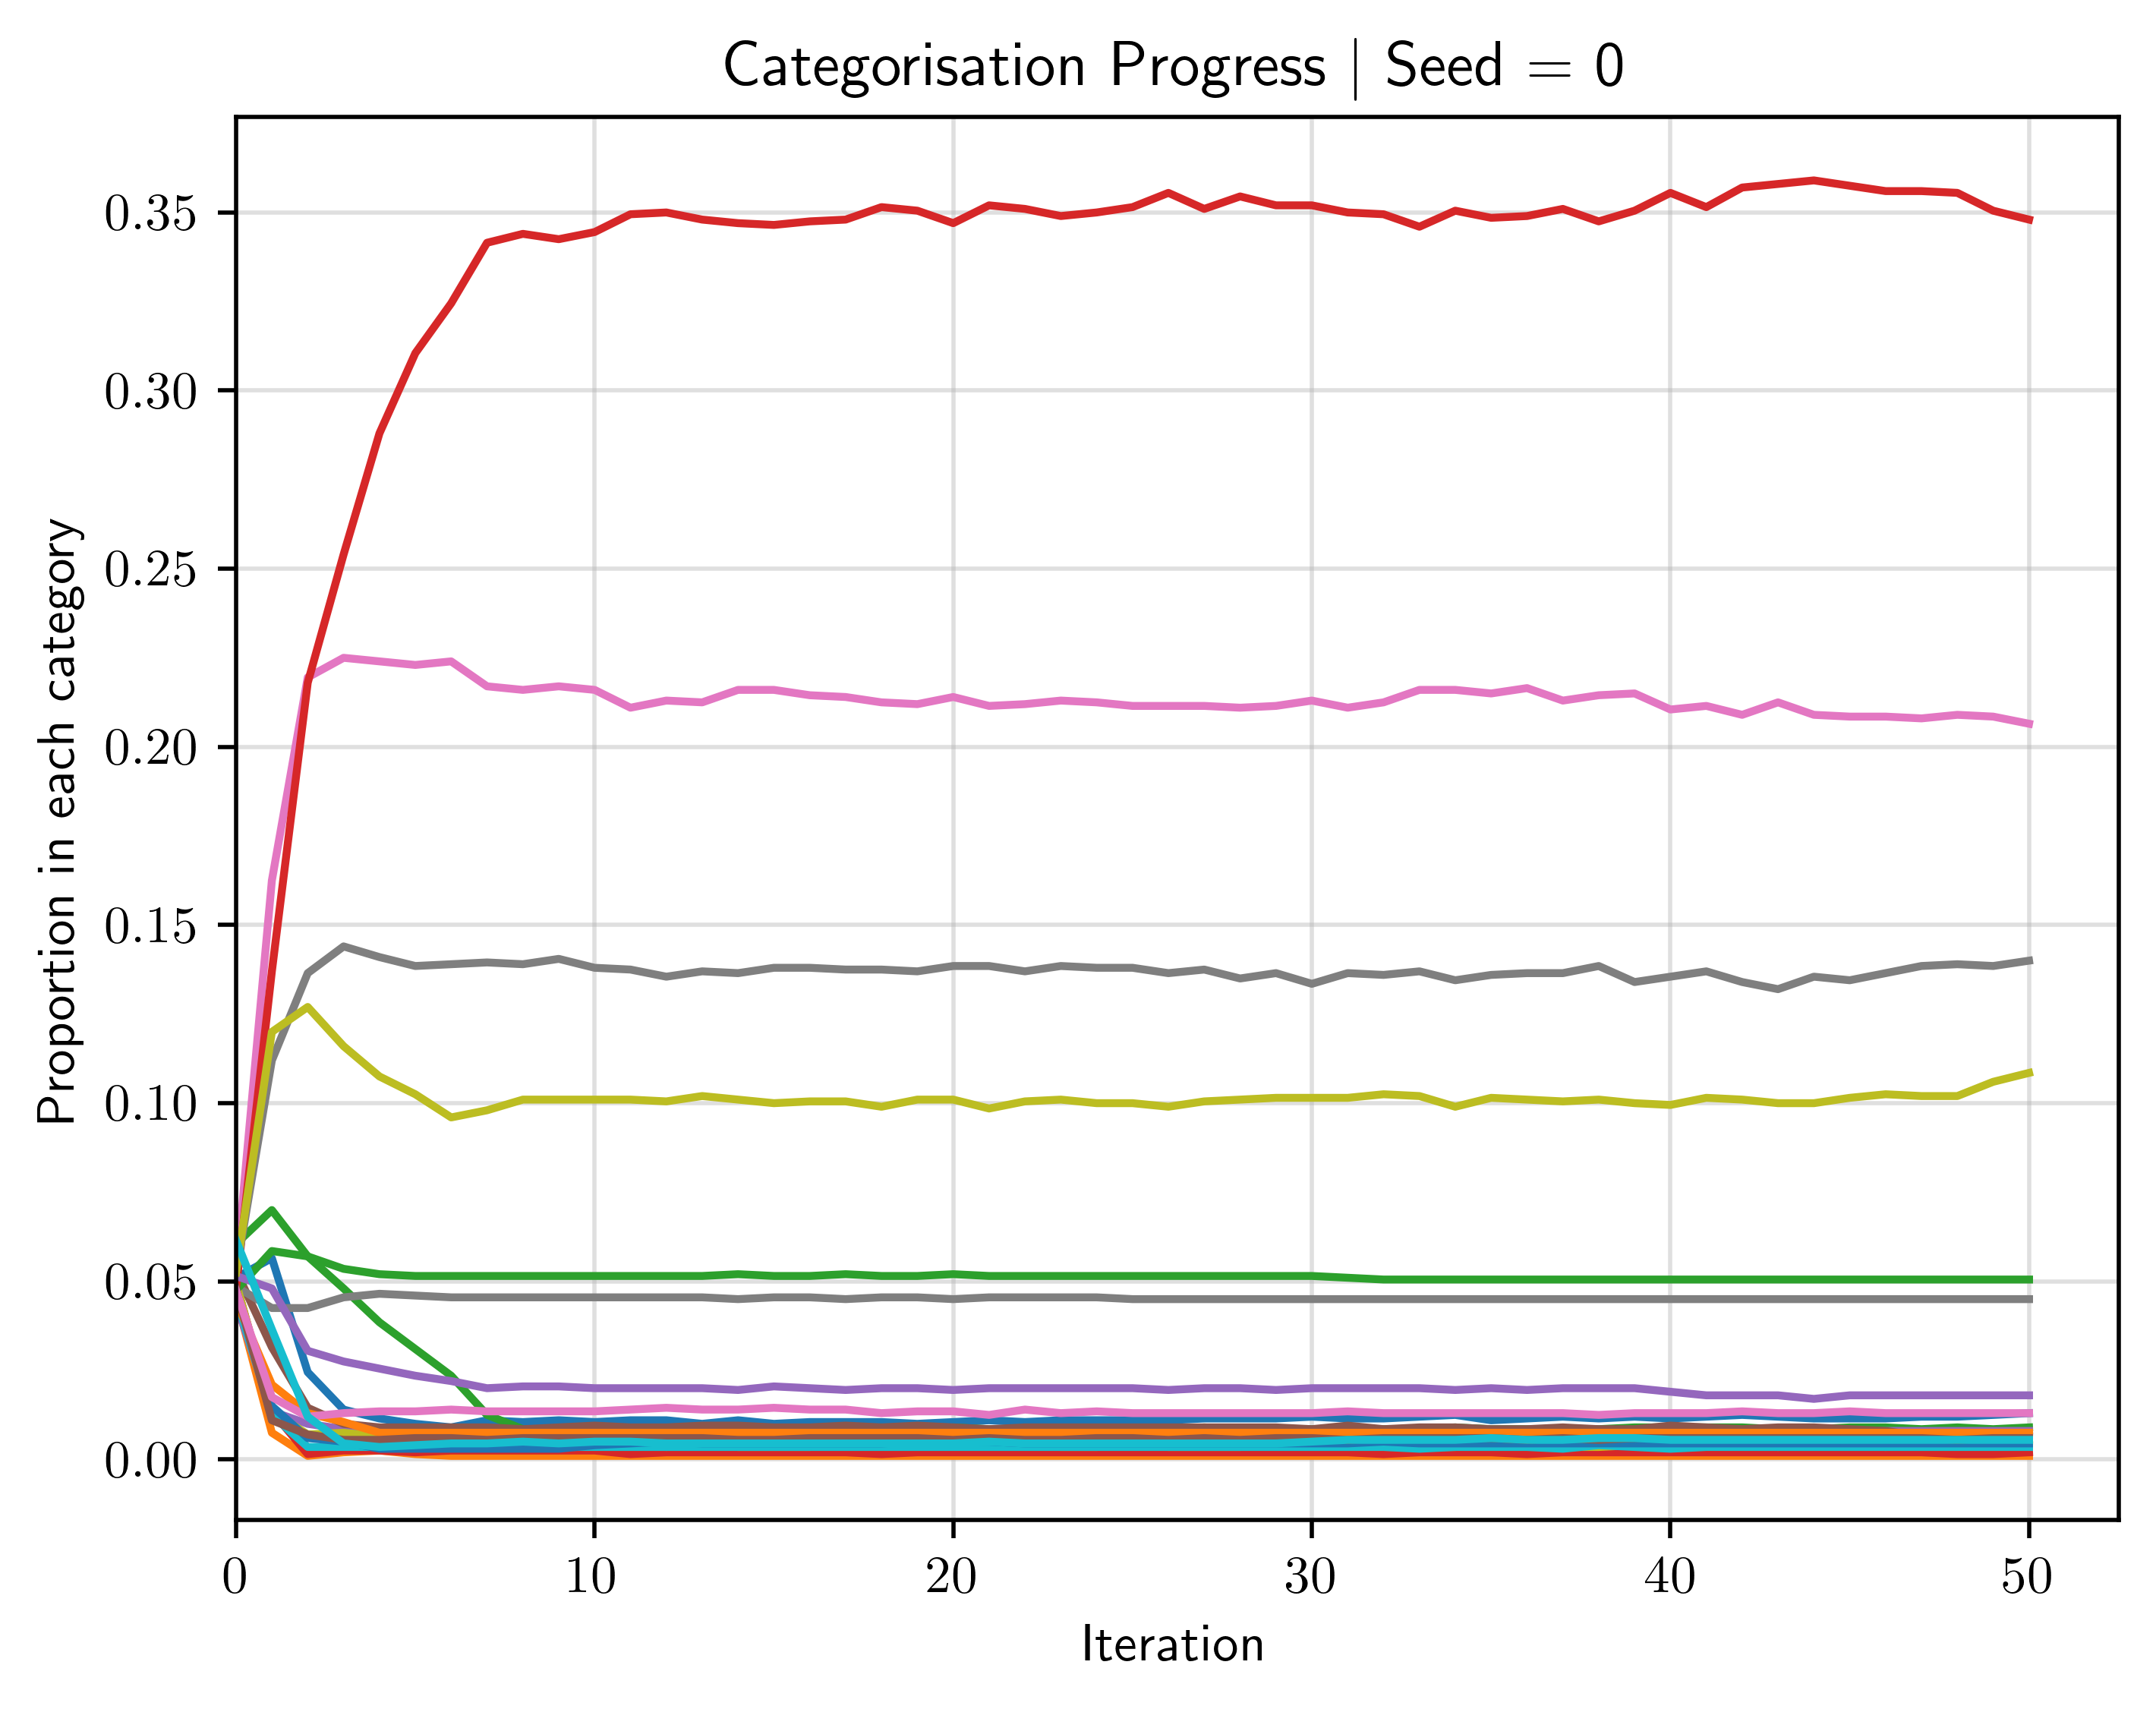
\includegraphics[width=0.99\textwidth]{../plots/d_progress_seed_0.png}
        \caption{Seed = 0}
    \end{subfigure}
    \hfill
    \begin{subfigure}[b]{0.32\textwidth}
        \centering
        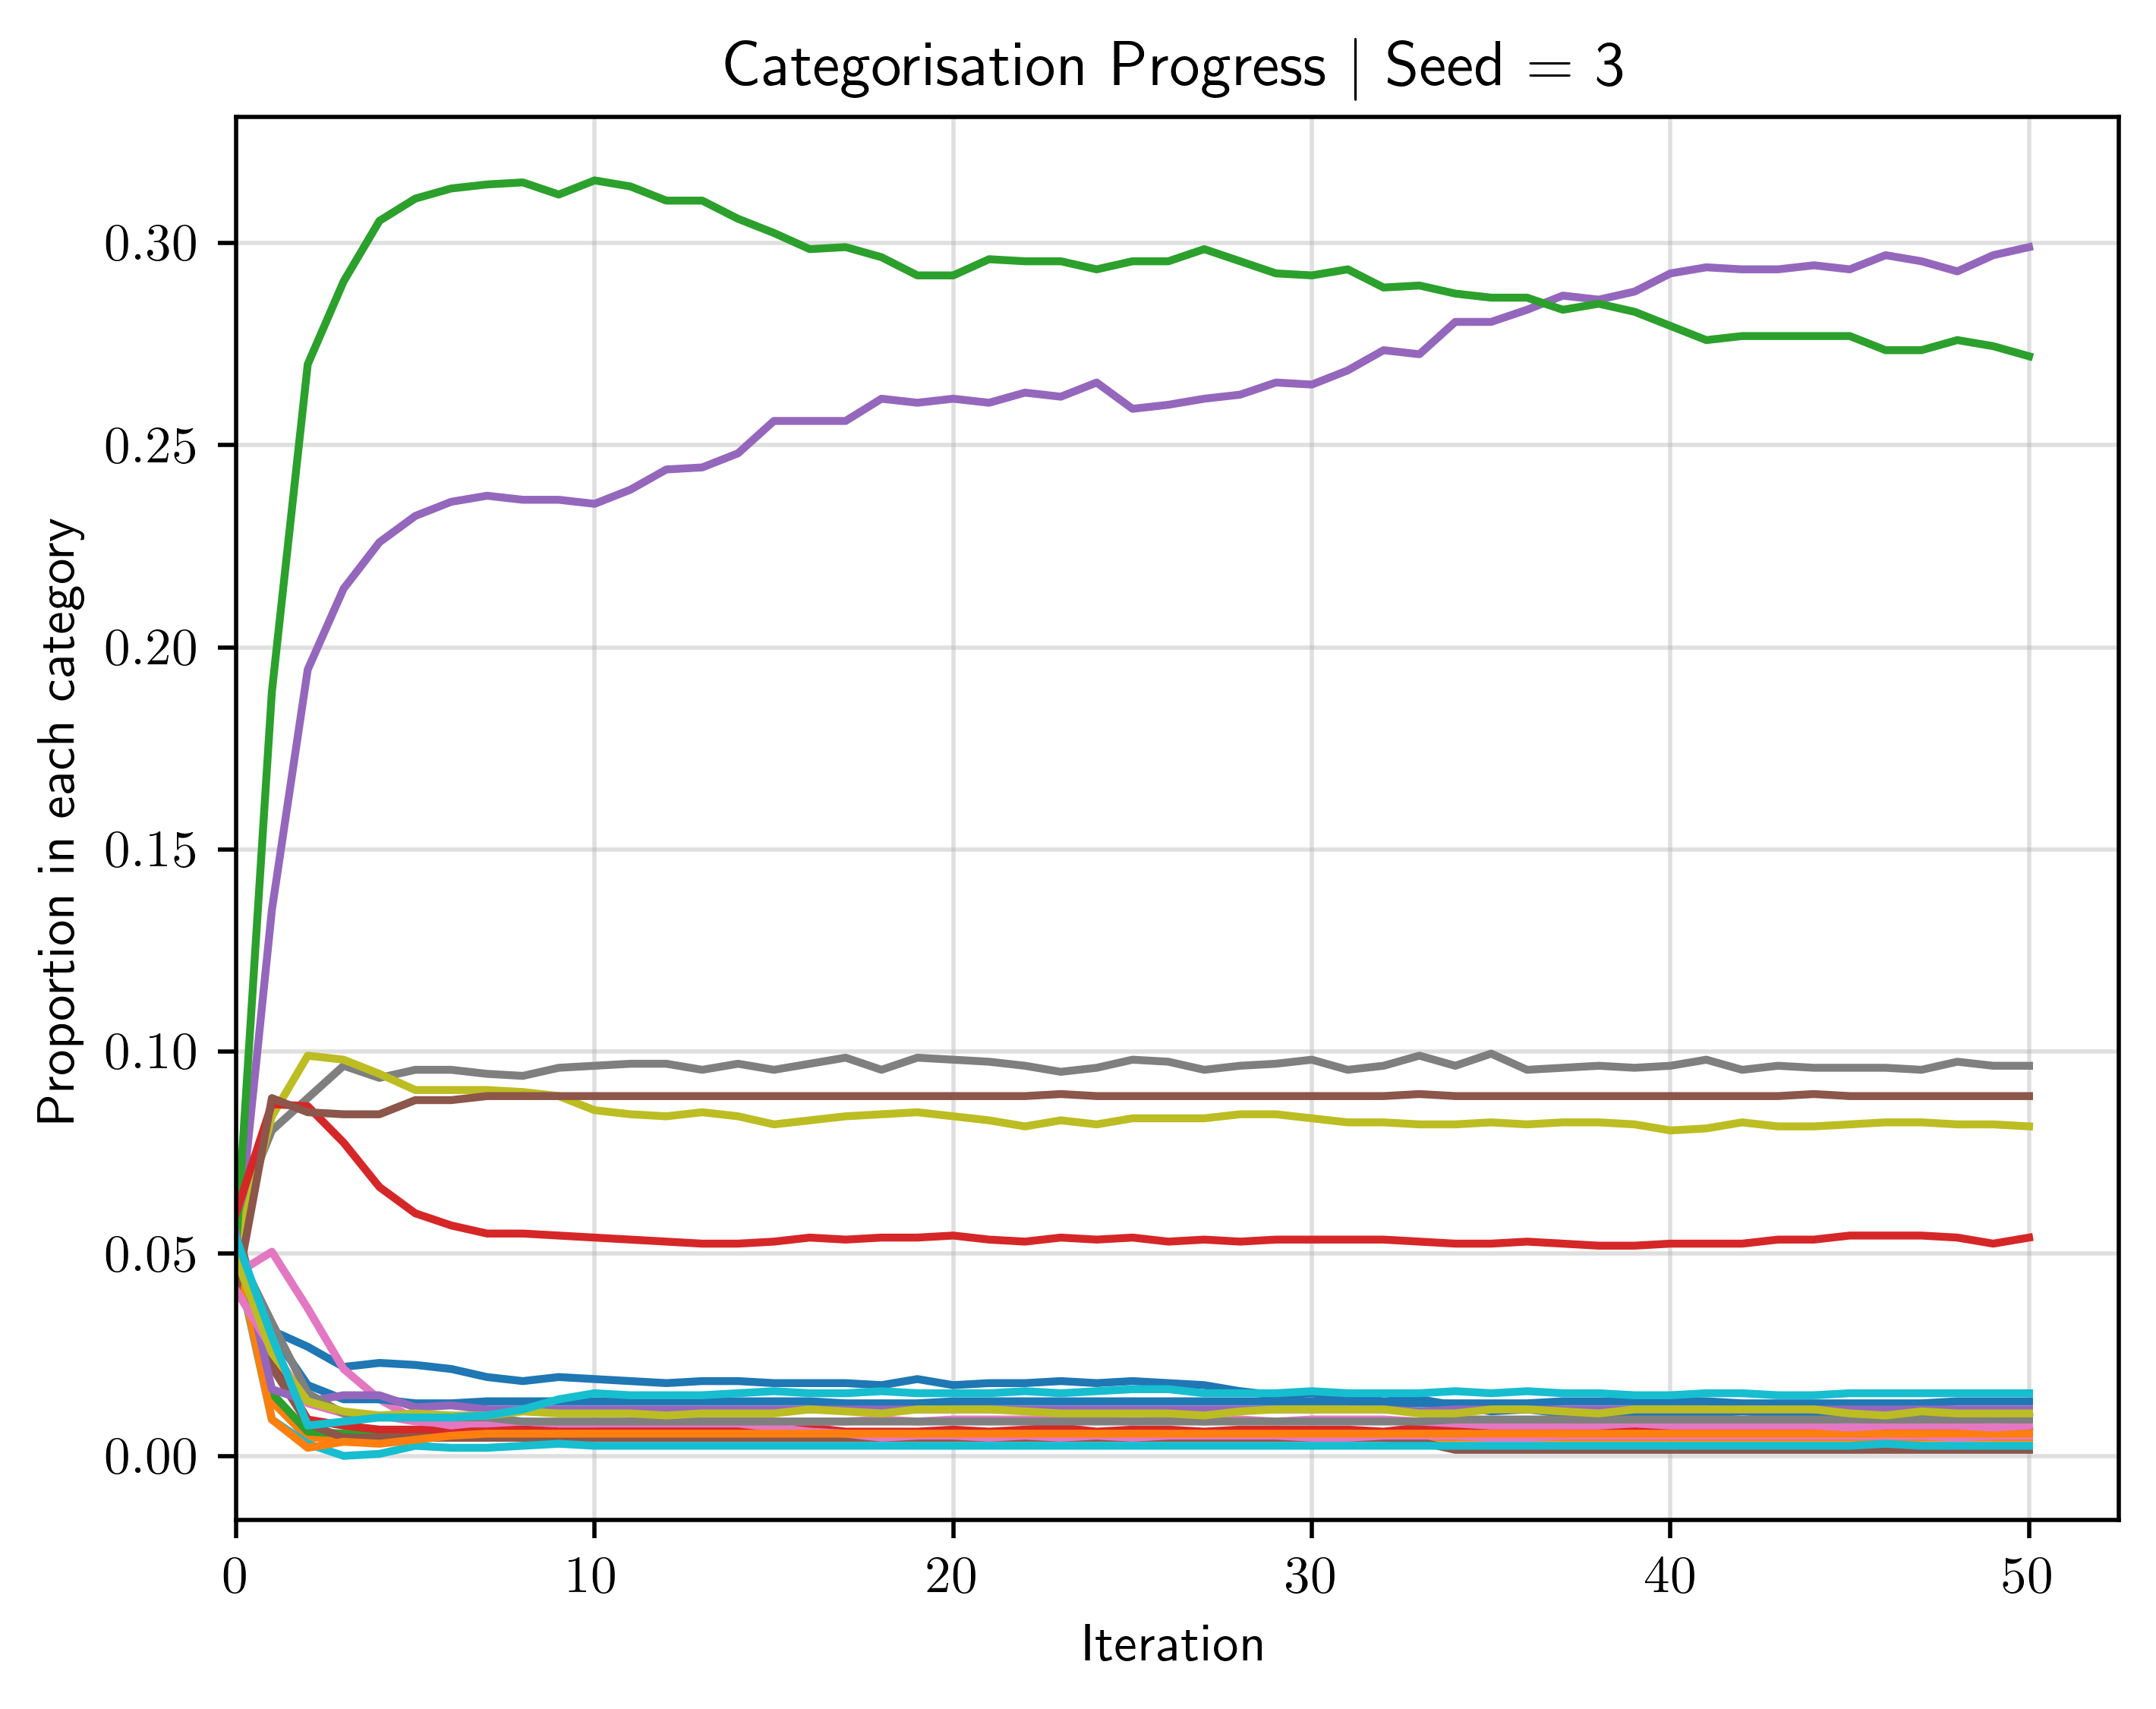
\includegraphics[width=0.99\textwidth]{../plots/d_progress_seed_3.png}
        \caption{Seed = 3}
    \end{subfigure}
    \hfill
    \begin{subfigure}[b]{0.32\textwidth}
        \centering
        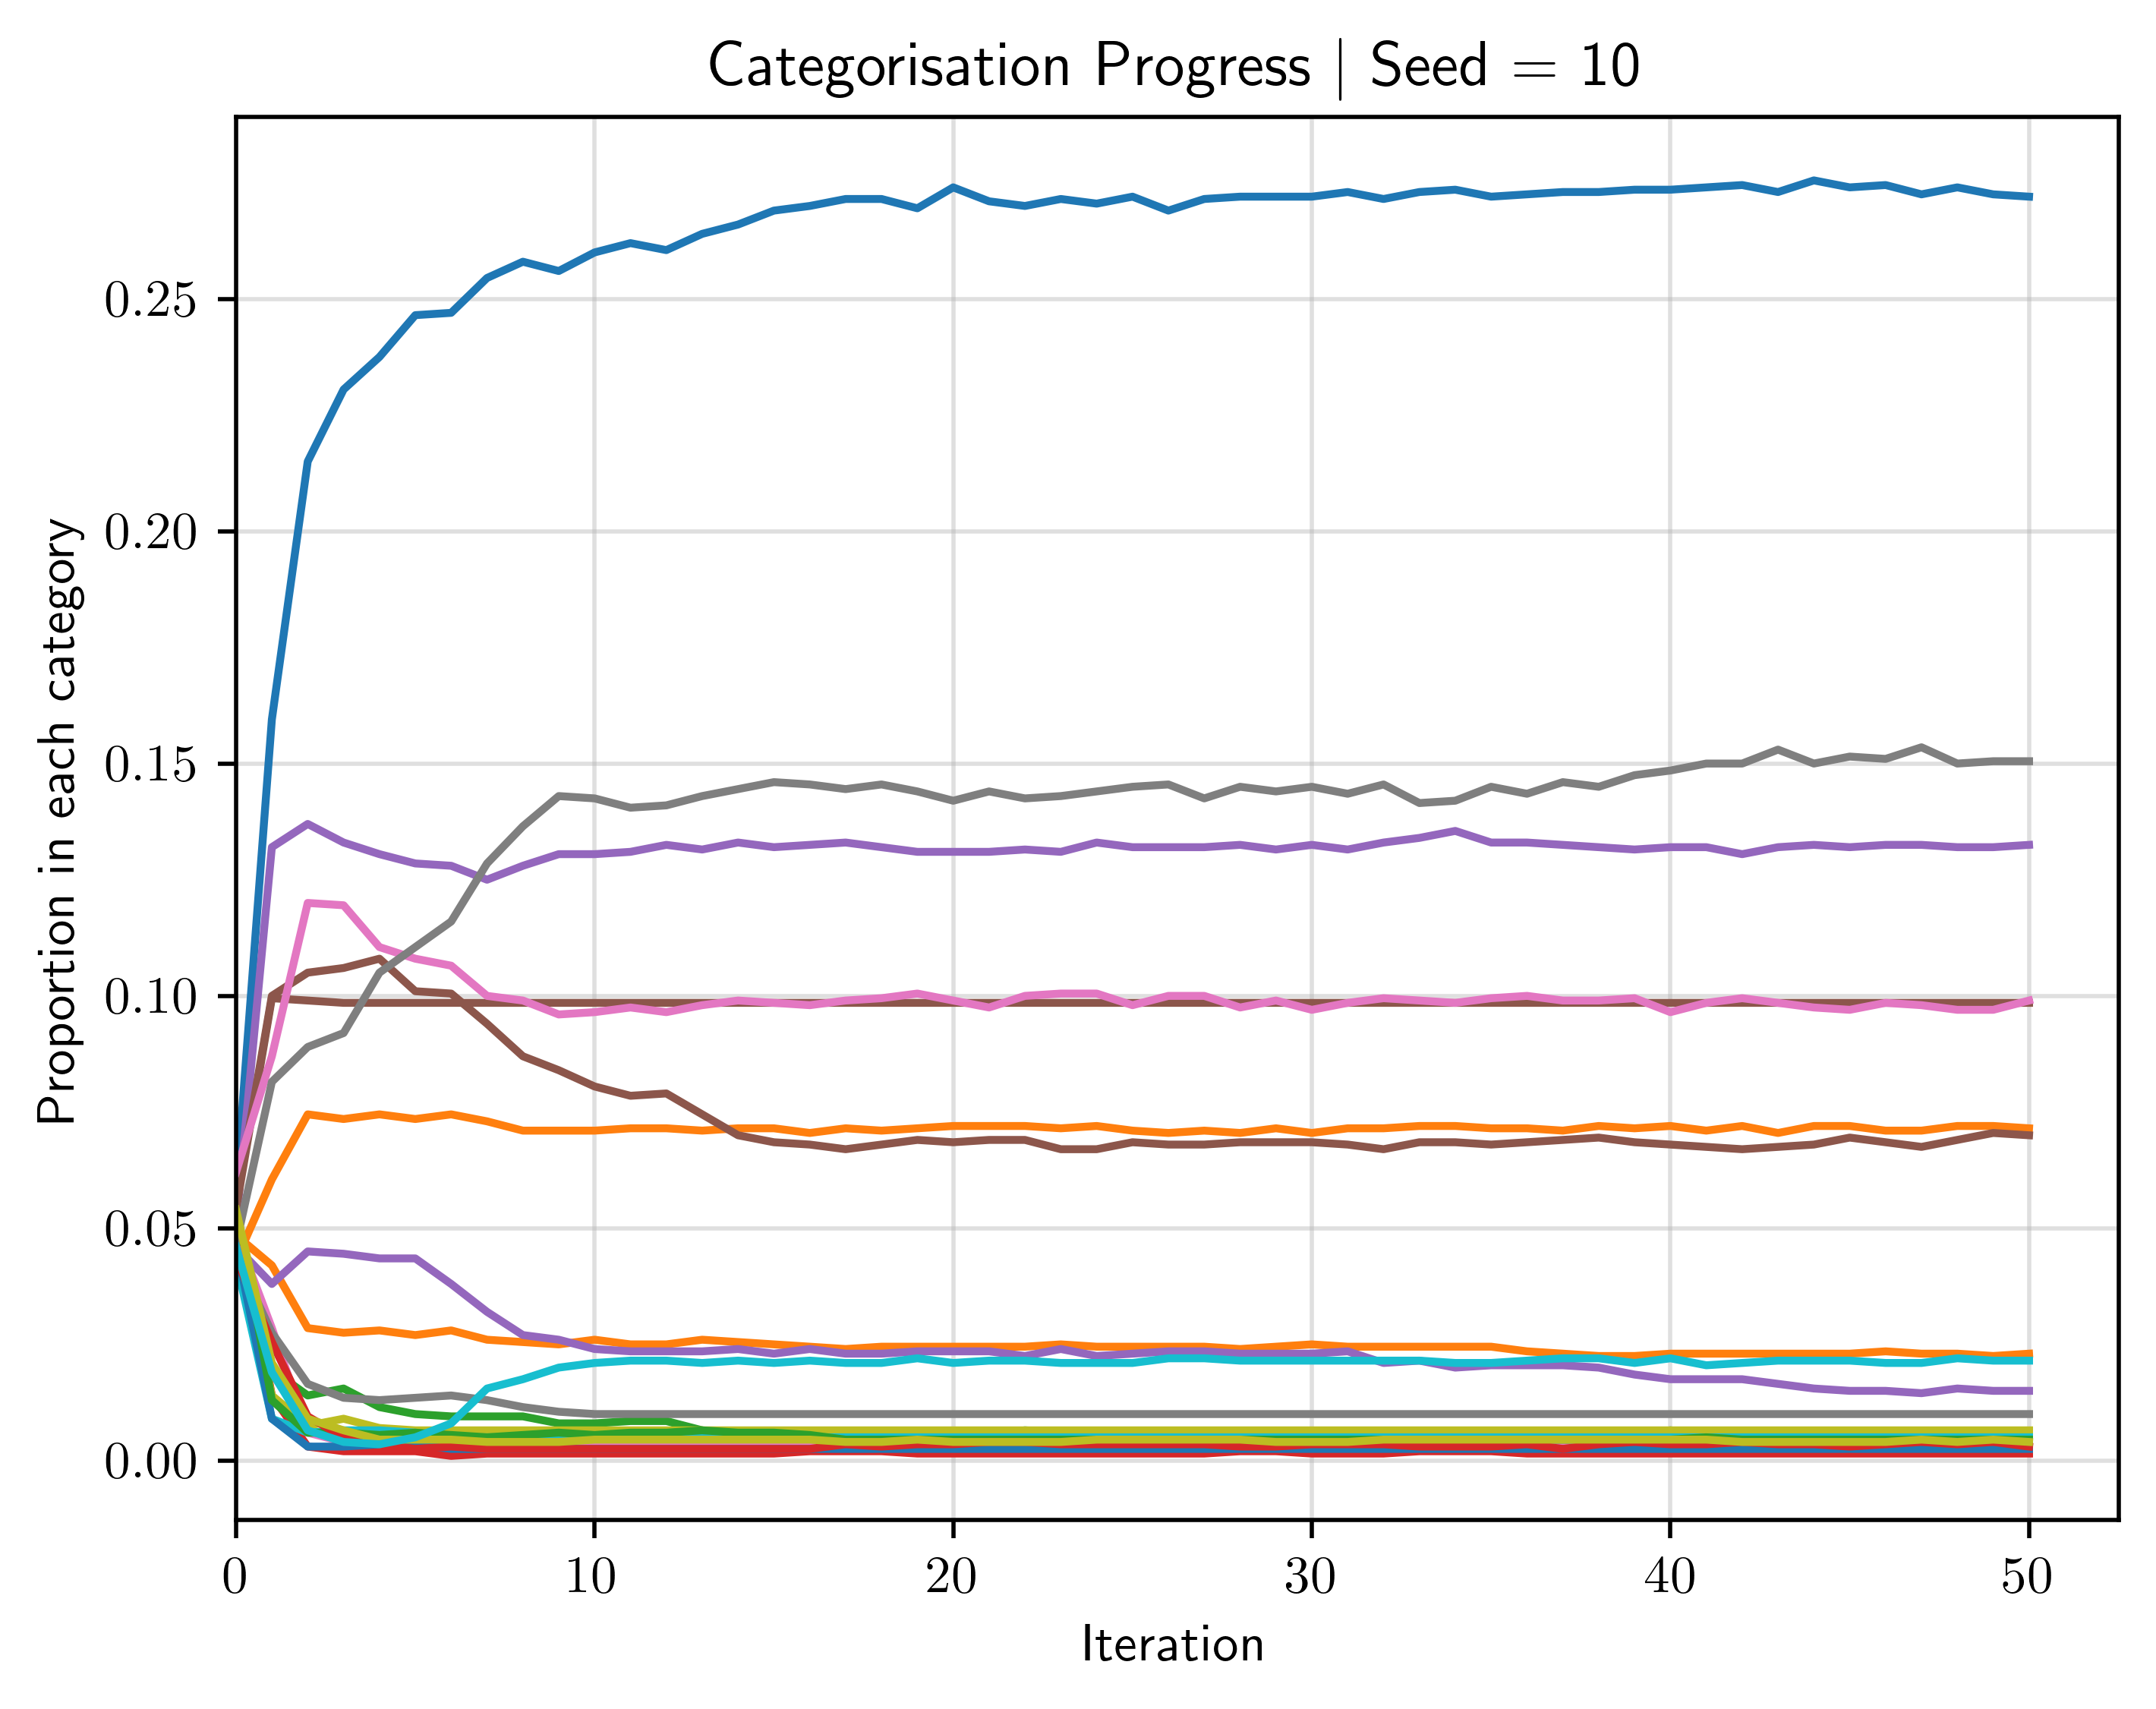
\includegraphics[width=0.99\textwidth]{../plots/d_progress_seed_10.png}
        \caption{Seed = 10}
    \end{subfigure}
    \caption{BMM Progress}\label{fig:taskd_all}
\end{figure}

Figure \ref{fig:taskd_all} shows the topic allocation progress for 3 different values of \verb|np.random.seed|.  For the most part, each reaches a stationary distribution, implying convergence of the model to a local minimum. However, different seeds yield different distributions, which are not explainable by relabelling. Also, the vast majority of the 20 clusters are pretty much ignored (i.e. the model does not ``believe'' there are 20 distinguishable clusters). It cannot therefore be said that the algorithm is finding the same global optimum each time, and therefore is not truly exploring the ``true'' posterior. However, the test set perplexities for the three seeds are 2111, 2124, and 2116, which (averaged) is a $\sim21$\% improvement over the model in Tasks B and C. Therefore the model must work well to a certain extent.

% seed = 0 gives 2111.419124109156
% seed = 3 gives 2123.59626206069
% seed = 10 gives 2115.947765676217



\section{Task E: Latent Dirichlet Allocation} \label{sec:e}
In Latent Dirichlet Allocation (LDA), each word in a document can be drawn from a different topic, and therefore each document now has its own distribution over topics $\bm{\theta}_d$. Figure \ref{fig:e_model} shows the model, and the difference between LDA and BMM can be seen as there is now a $\bm{\theta}_d$ for each document, rather than only one $\bm{\theta}$ for the whole model. This increases the number of parameters significantly, making the need for Gibbs Sampling greater.

\begin{figure}[h]
    \centering
    \makebox[\textwidth]{
        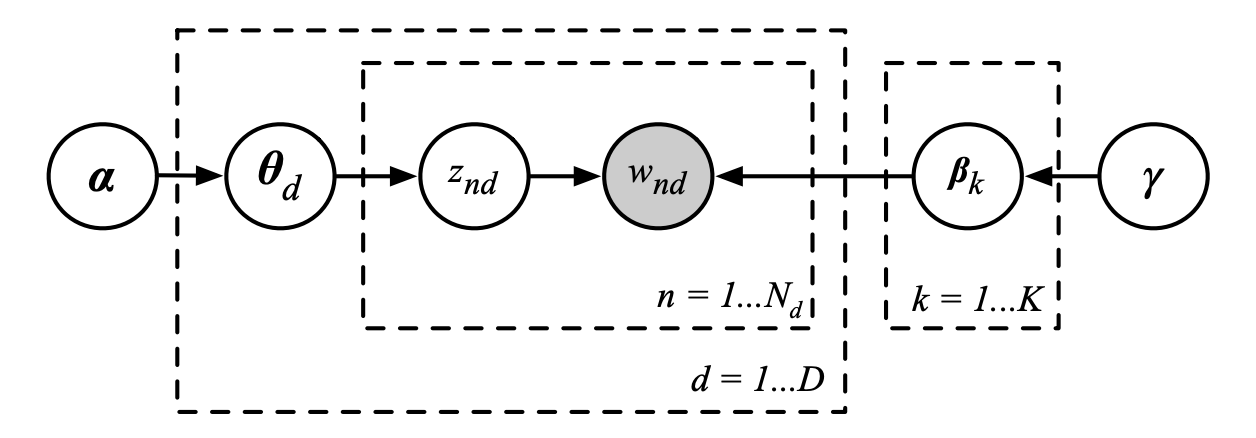
\includegraphics[width=0.5\textwidth]{../plots/Screenshot 2023-11-30 at 23.39.08.png}
    }
    \caption[Latent Dirichlet Allocation Model]{Latent Dirichlet Allocation Model\protect\footnotemark} \label{fig:e_model}
\end{figure}
\footnotetext{See Footnote \ref{fn:l_notes}}

The provided python function \verb|LDA| was modified in a similar way to in Task D to return the topic posteriors at each Gibbs iteration, and also to return the word entropies for each topic at each iteration.

The model was run with parameters $\alpha =0.1, \gamma = 0.1$ as before, giving a per-word perplexity of 1644, by far the lowest of all the models so far. This is as desired - we are increasing the complexity of the model but still decreasing the log likelihood of the test set - therefore the model is not overfitting to the training set.

Figure \ref{fig:taske_thetas} shows the topic posteriors as a function of the Gibbs iteration for 3 different documents. The Gibbs sampler exhibits the \emph{rich get richer} property - the more words in a document already assigned to a topic, the more a word is likely to be assigned to that topic. This explains why each document has one topic than dominates. It is possible that more than 50 iterations would be useful, as the topic allocations do not seem to have reached a stationary distribution. It was unfortunately not possible to run for more than 50 iterations to test this as the function was taking over 30 minutes to run.

The oscillations that persist may also be due to high similarity between multiple topics, which could be due to having too many topics, meaning a word has a similar probability of being drawn into either topic.

\begin{figure}[h]
    \centering
    \makebox[\textwidth]{
        \begin{subfigure}[b]{0.35\textwidth}
            \centering
            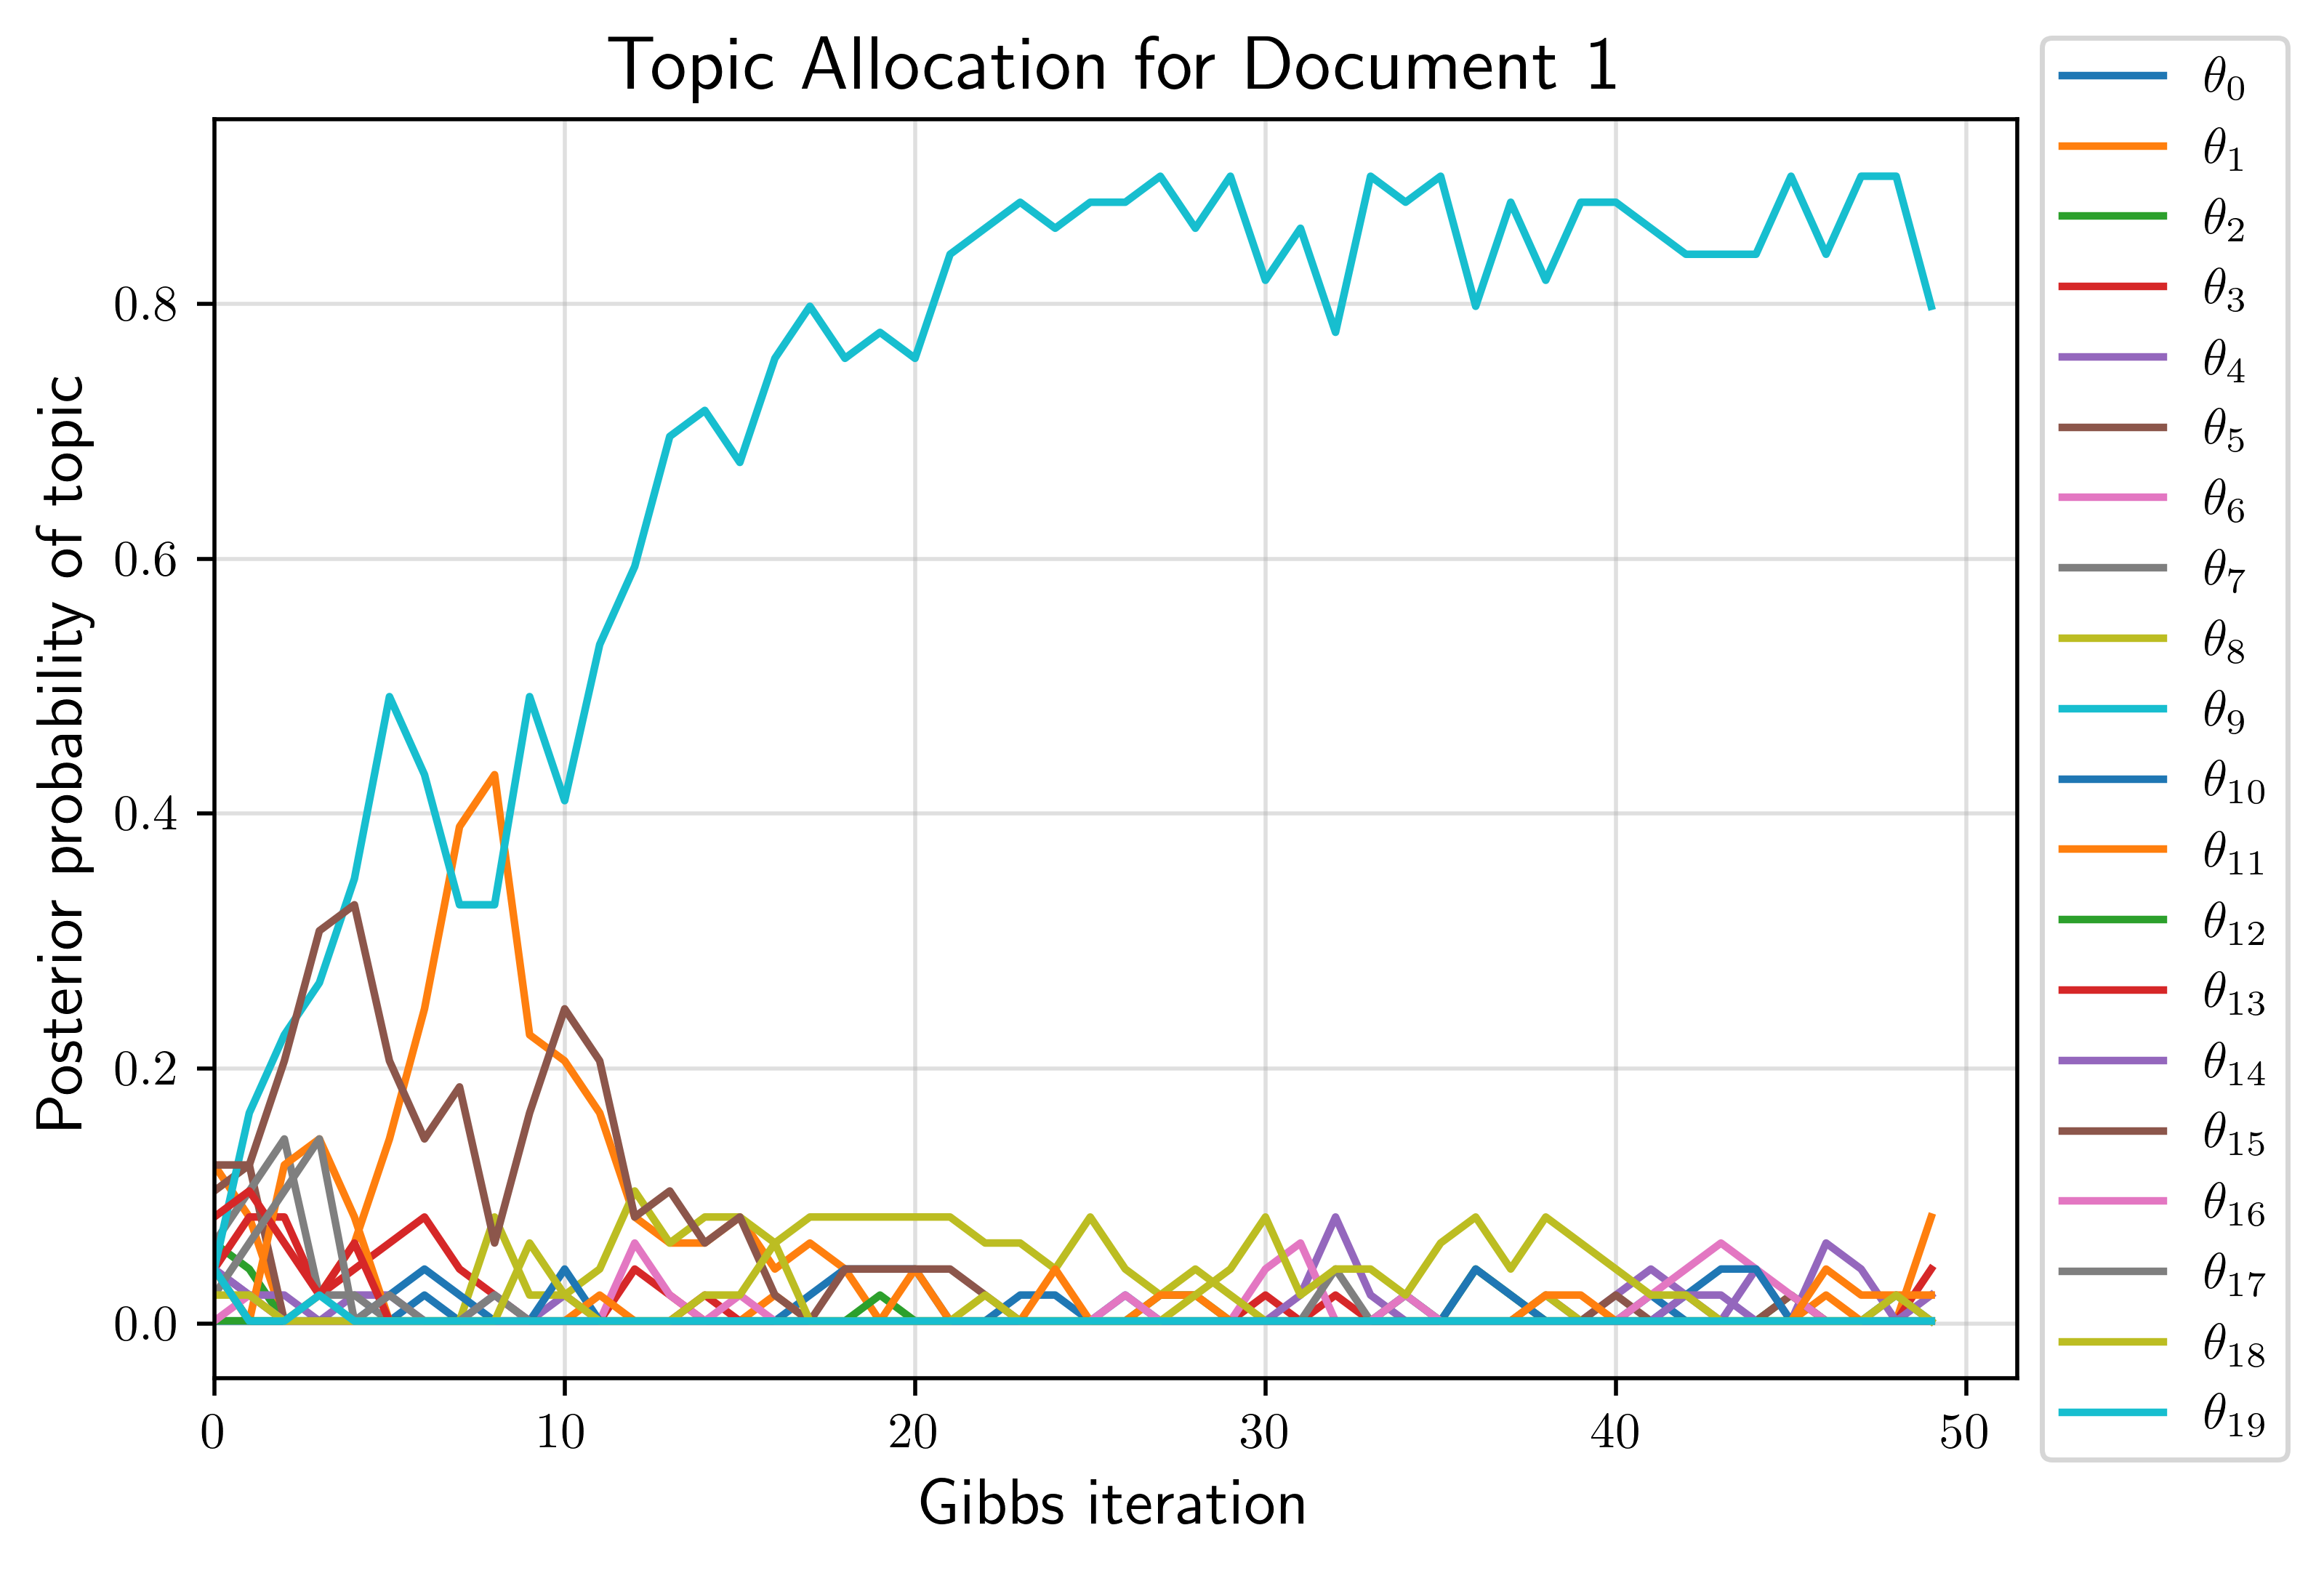
\includegraphics[width=0.99\textwidth]{../plots/e_thetas_doc_1.png}
            \caption{Document 1}
        \end{subfigure}
        \hfill
        \begin{subfigure}[b]{0.35\textwidth}
            \centering
            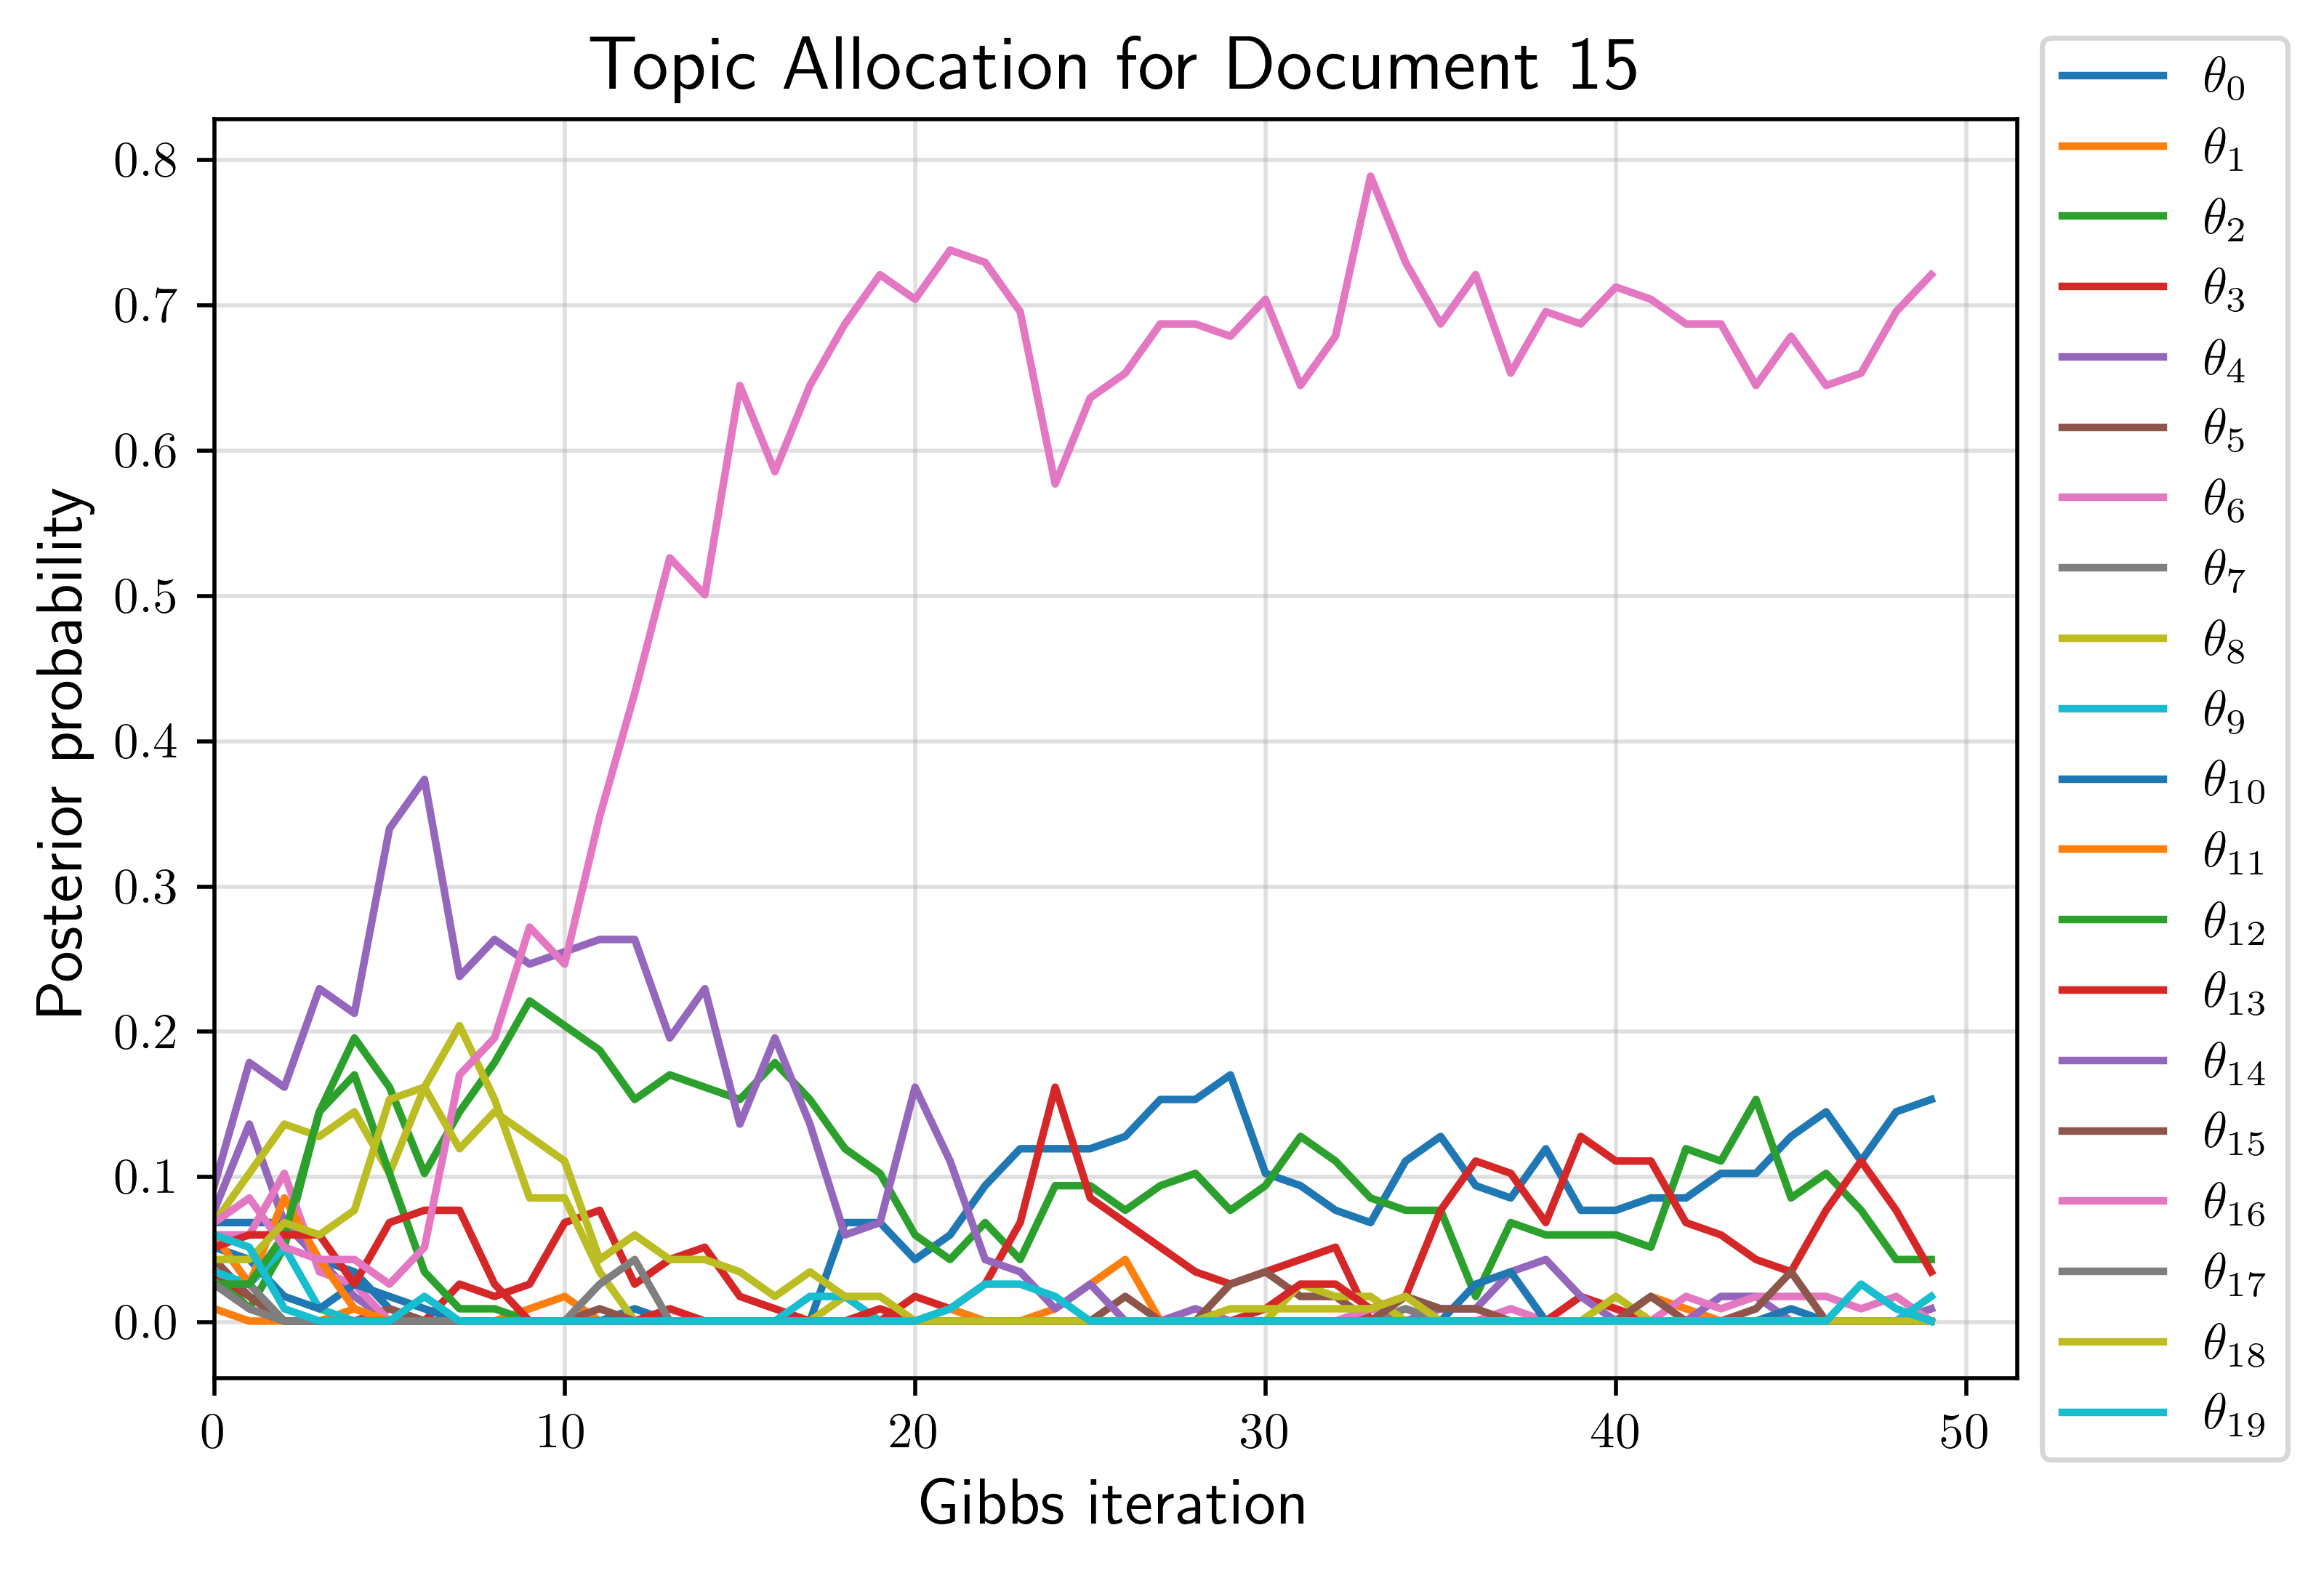
\includegraphics[width=0.99\textwidth]{../plots/e_thetas_doc_15.png}
            \caption{Document 15}
        \end{subfigure}
        \hfill
        \begin{subfigure}[b]{0.35\textwidth}
            \centering
            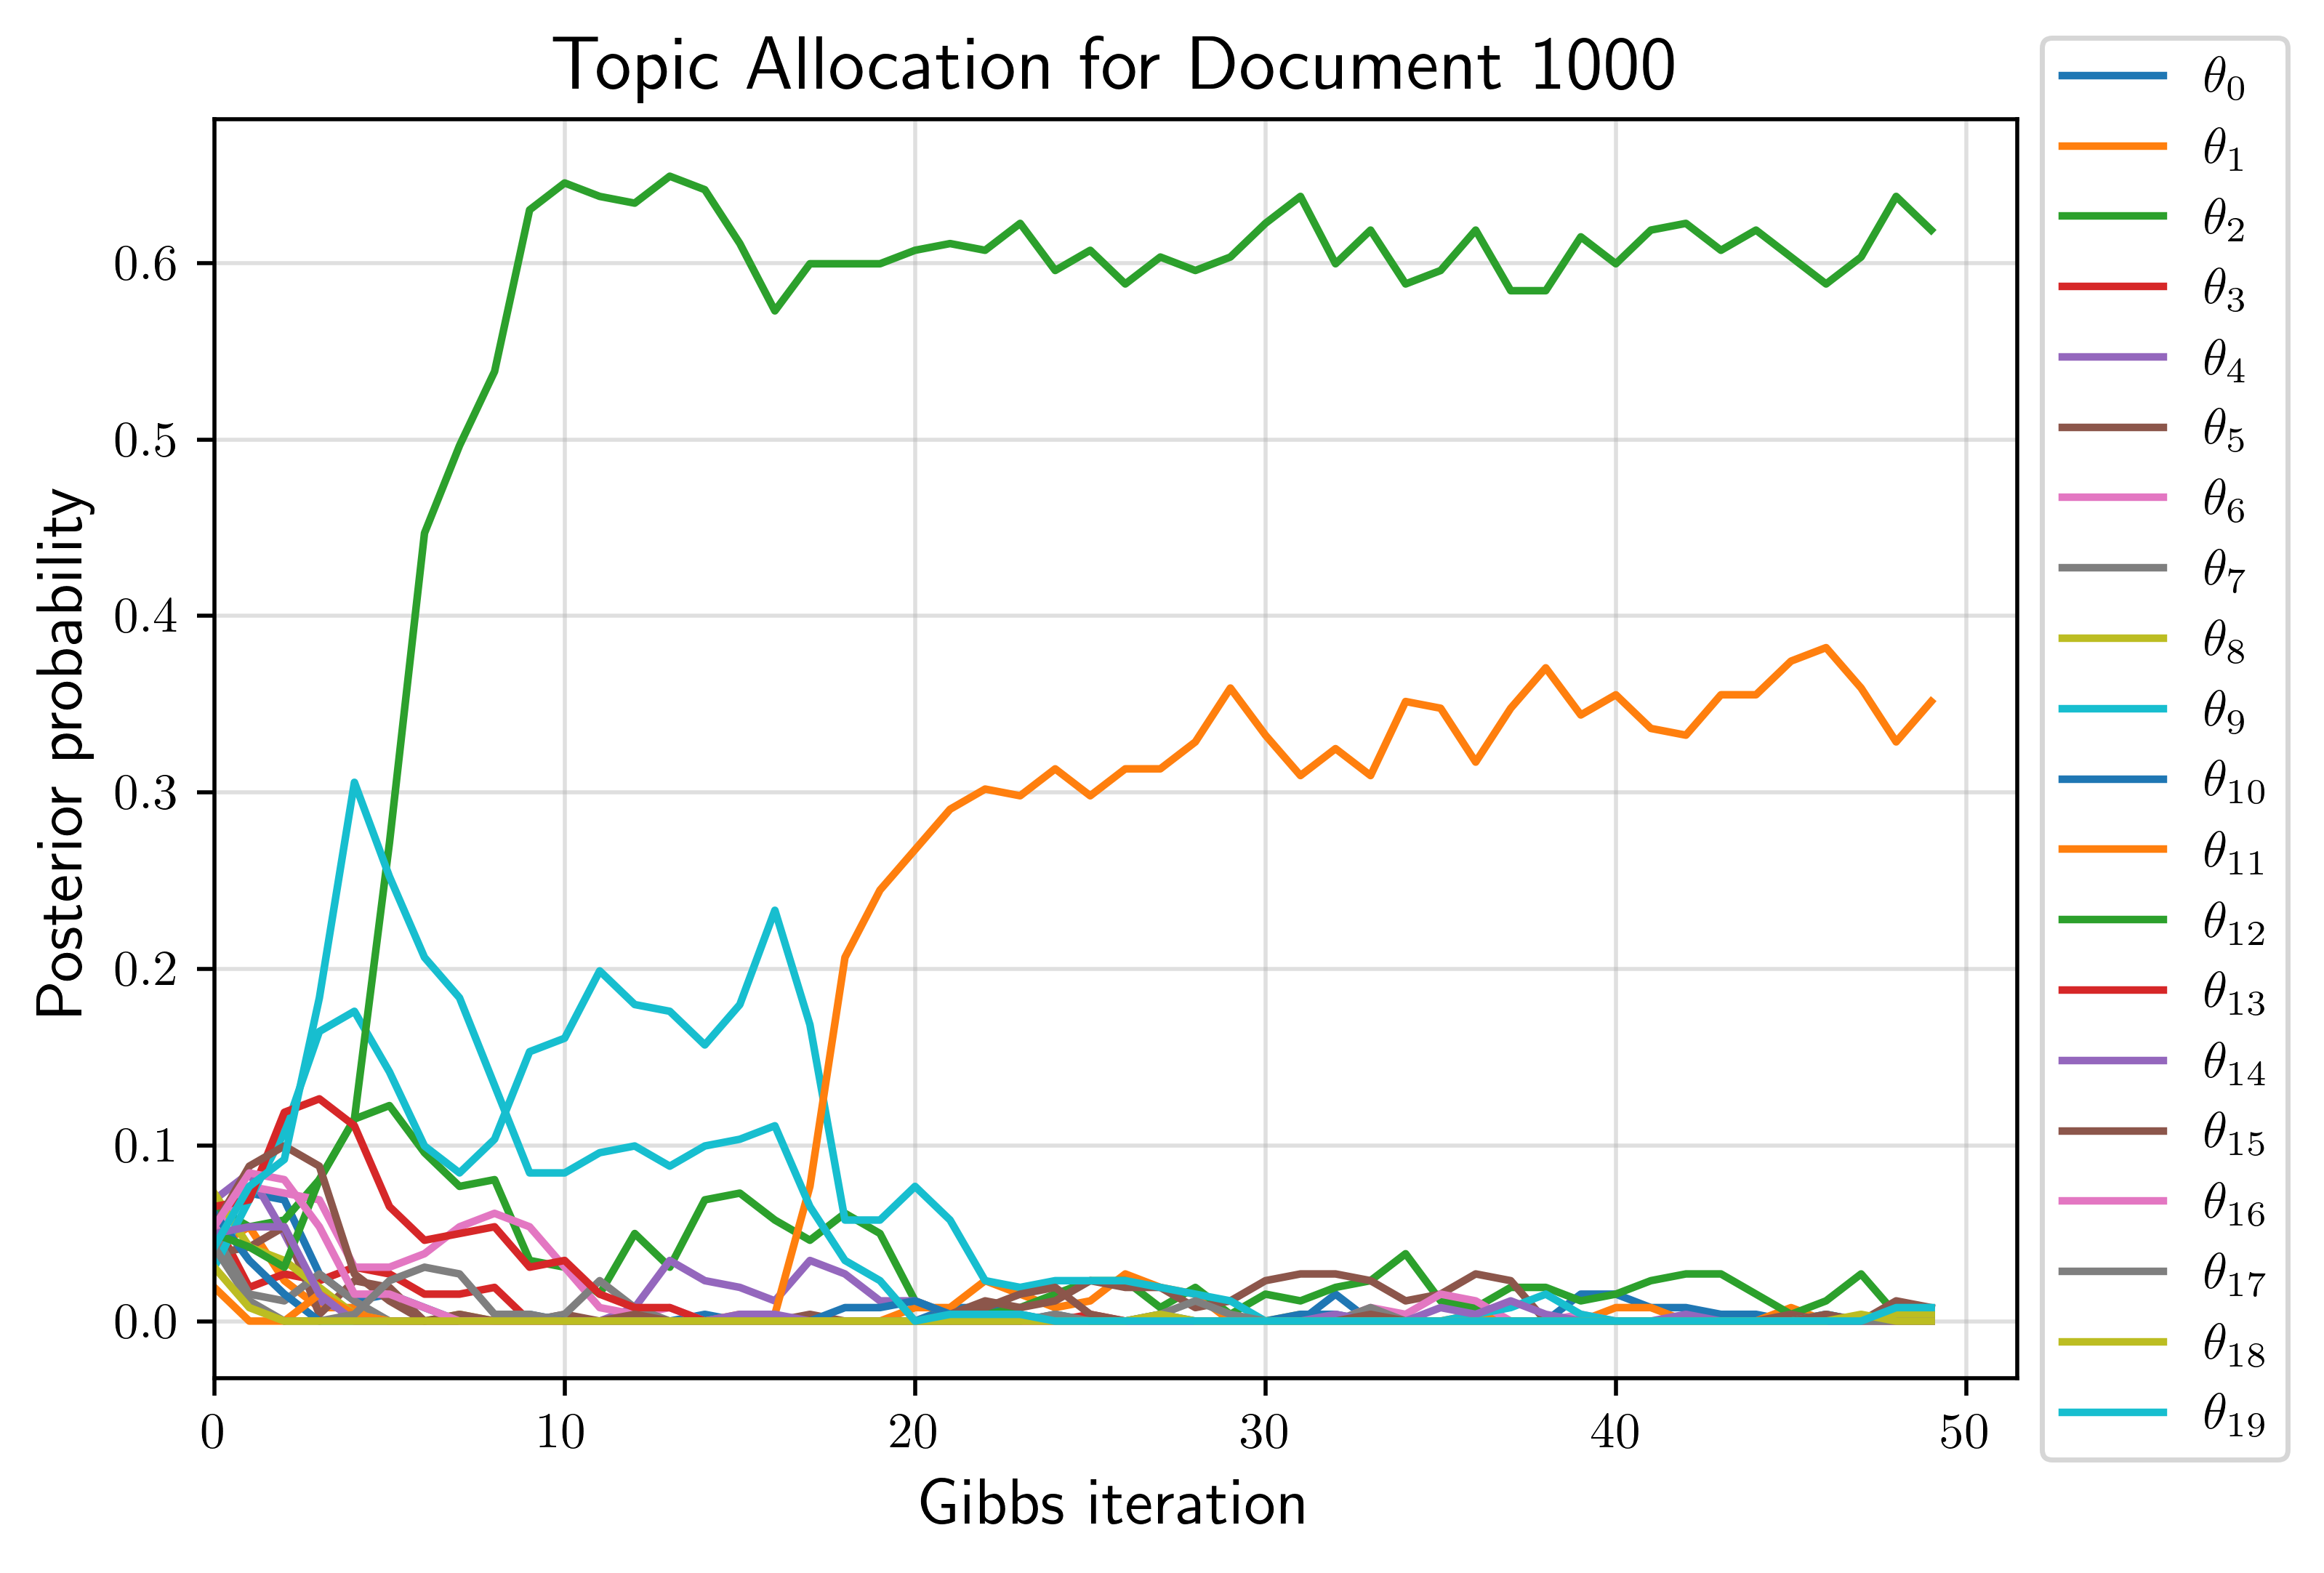
\includegraphics[width=0.99\textwidth]{../plots/e_thetas_doc_1000.png}
            \caption{Document 354}
        \end{subfigure}}
    \caption{LDA Topic Progress}\label{fig:taske_thetas}
\end{figure}

The word entropy can be calculated using equation \ref{eqn:e_entropy}. This is the expected uncertainty associated with each observation. Figure \ref{fig:e_entropies} shows the word entropies for each topic against the Gibbs iteration. Initially, all the topics have the same entropy. After some iterations the entropy decreases, as the topics are reaching a distinct, non-uniform distribution - the topics are becoming more specific as training occurs, as expected. This means fewer words are required to ``describe'' the topic, or the topic has a smaller vocabulary - therefore the entropy decreases. The entropies reach fairly stable values after 50 iterations, implying that not many, if any, more iterations are required to train the model any better.

\begin{equation} \label{eqn:e_entropy}
    H_k = -\sum_{m=1}^{M}\beta_{km}\log(\beta_{km})
\end{equation}

The natural logarithm is used instead of the standard base 2 logarithm as that allows for easier comparison with the perplexity. Using the natural logarithm results in units of nats, not bits. The log-perplexity is a comparable unit to the entropy, as they will be the the same if measuring an infinitely long document on a single topic. The log-perplexity of the test set is $\log1644= 7.40$, which is higher than all the topic entropies, as expected as the test set is a blend of all the topics, and therefore less specific than any single topic.
\begin{figure}[h]
    \centering
    \makebox[\textwidth]{
        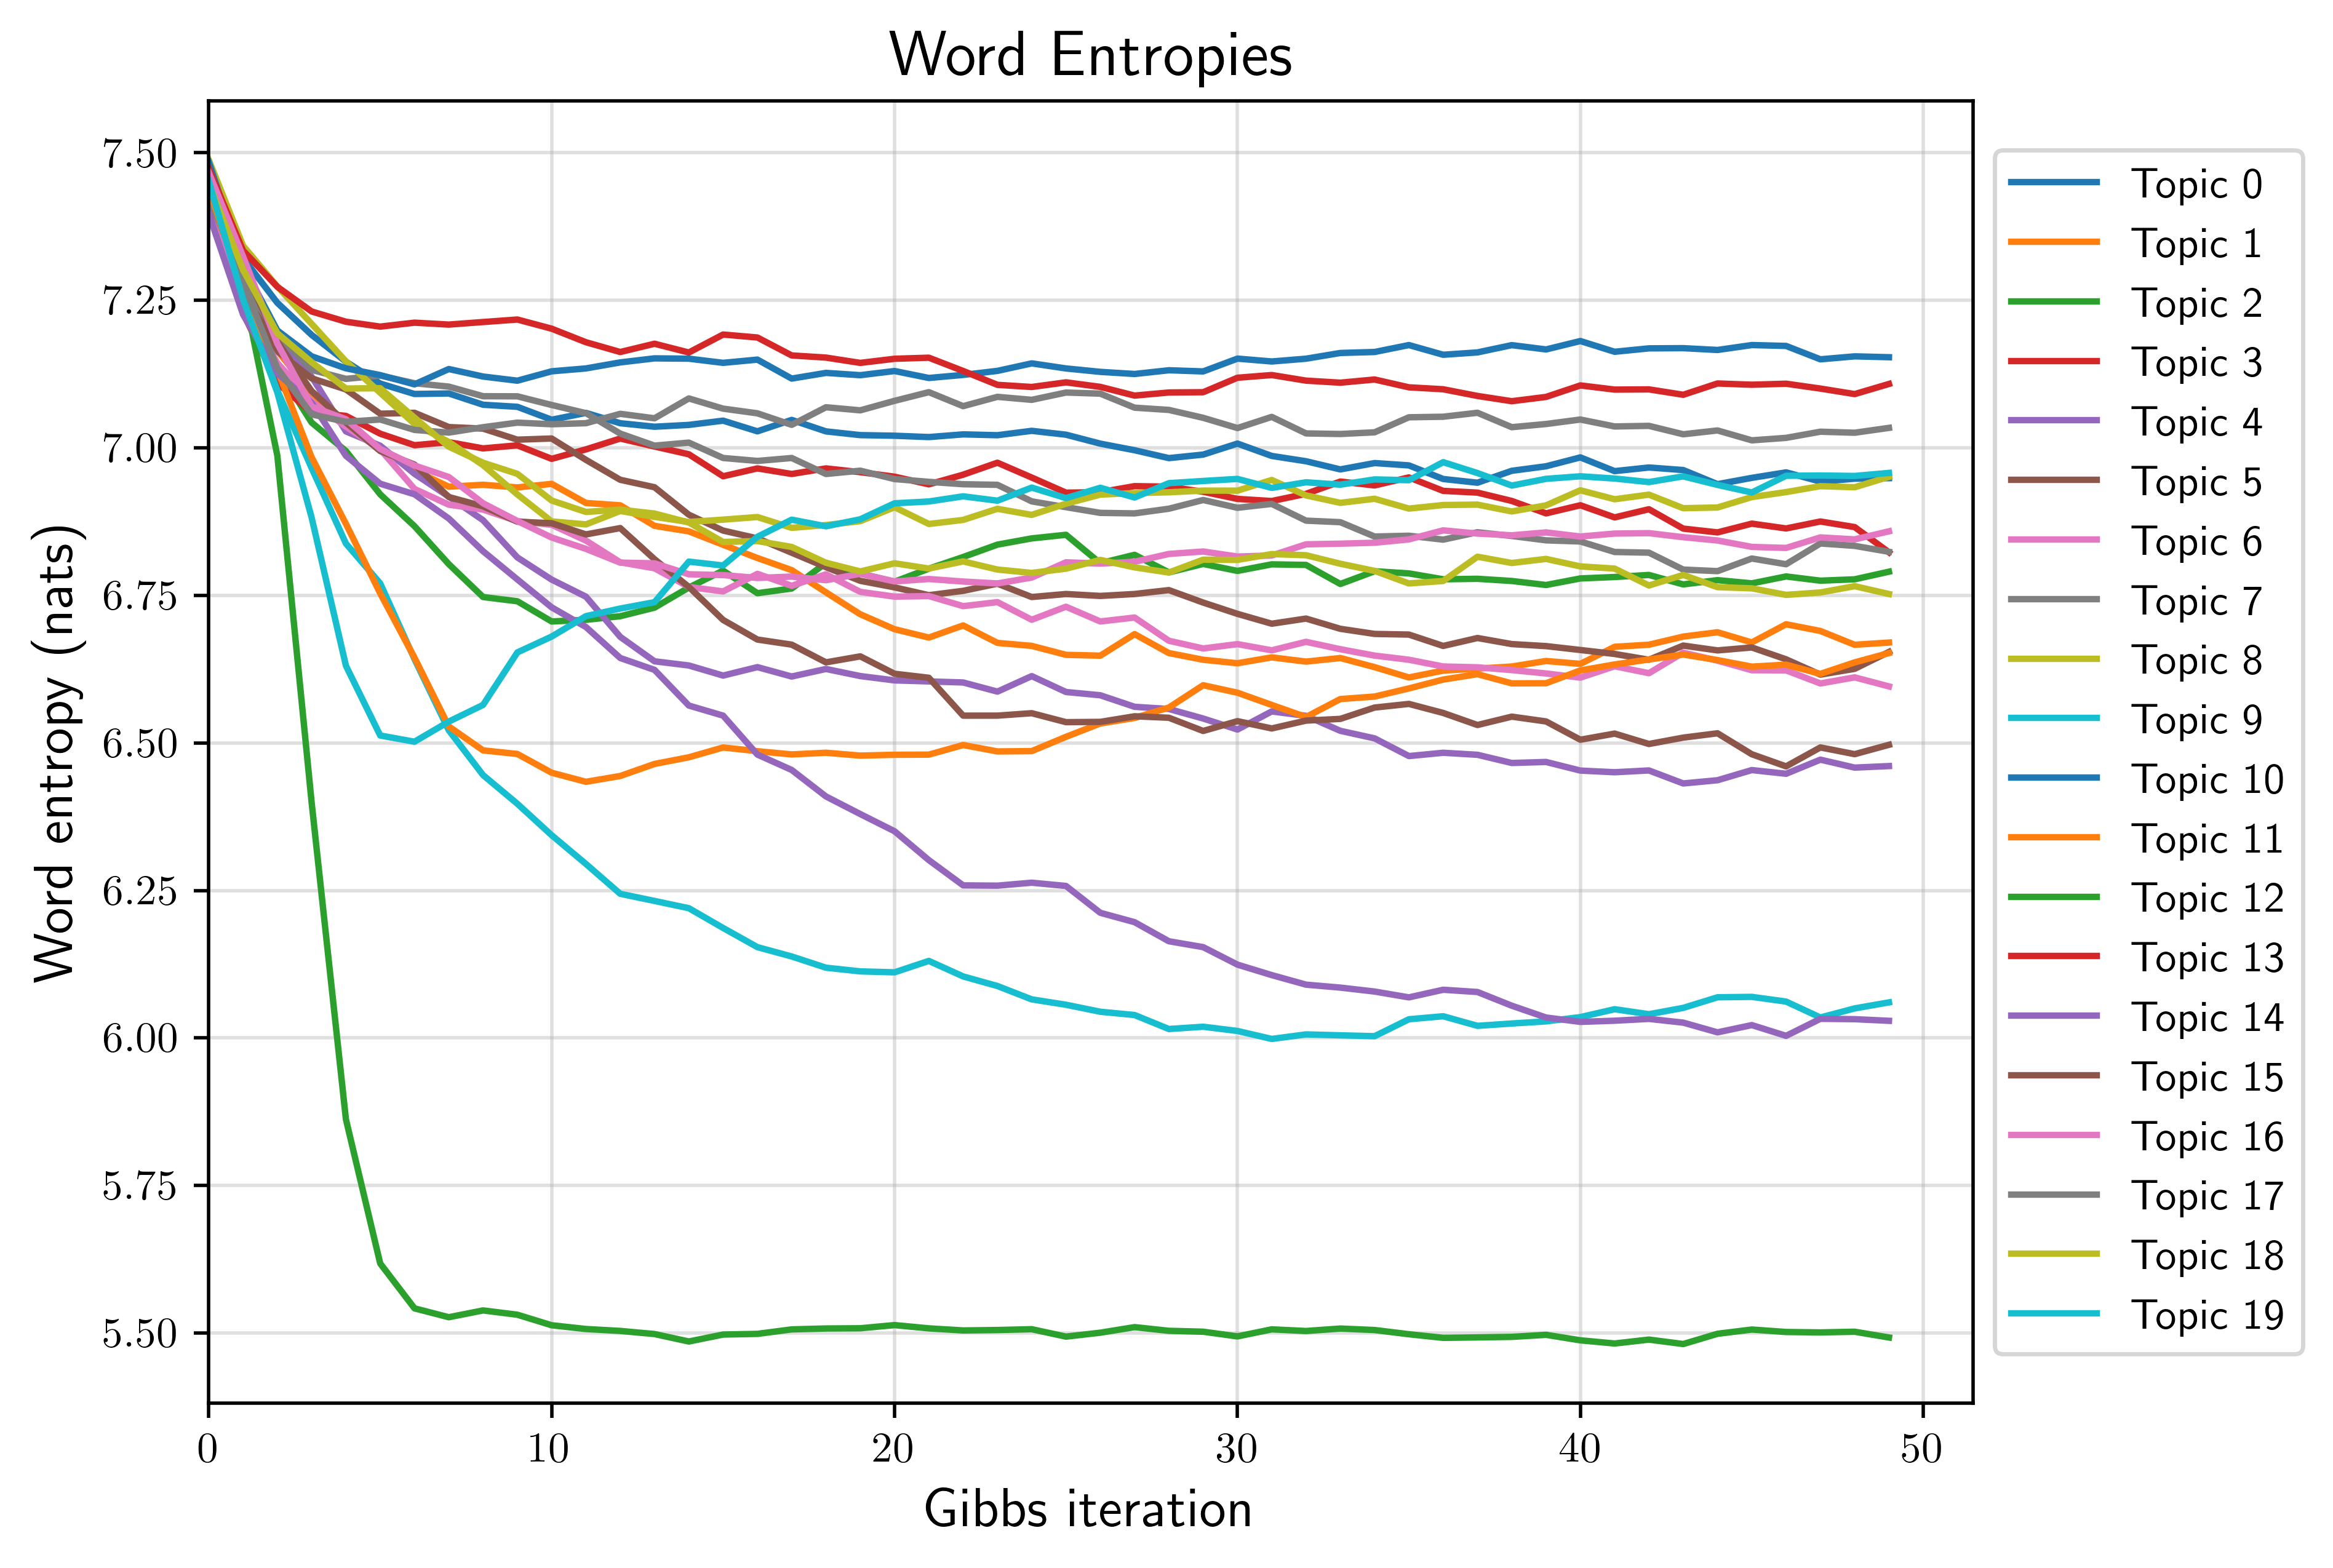
\includegraphics[width=0.5\textwidth]{../plots/e_entropies.png}
    }
    \caption{Entropy Evolution} \label{fig:e_entropies}
\end{figure}



% \begin{eqnarray}
%     p(w_i > w_j) = p(w_j-w_i < 0) =\Phi \left(\frac{\mu_i - \mu_j}{\sqrt{\lambda_i^{-1} + \lambda_j^{-1}}}\right) \\ \label{eqn:skilldiff}
%     p(w_i - w_j + n > 0) = \Phi \left(\frac{\mu_i - \mu_j}{\sqrt{\lambda_i^{-1} + \lambda_j^{-1} + 1}}\right) \label{eqn:win}
% \end{eqnarray}



% \begin{table}
%     \centering{}
%     \begin{minipage}[t]{0.495\textwidth}
%         \begin{center}
%             \begin{tabular}{lcccc}\toprule
%                 ---         & D           & N           & F           & M           \\ \midrule
%                 Djokovic(D) & \num{0.500} & \num{0.940} & \num{0.909} & \num{0.985} \\
%                 Nadal(N)    & \num{0.060} & \num{0.500} & \num{0.427} & \num{0.767} \\
%                 Federer(F)  & \num{0.091} & \num{0.573} & \num{0.500} & \num{0.811} \\
%                 Murray(M)   & \num{0.015} & \num{0.233} & \num{0.189} & \num{0.500} \\  \bottomrule
%             \end{tabular}%
%             \par\end{center}
%         \caption{p(Higher Skill)} \label{tab:skill_prob}
%         %
%     \end{minipage}%
%     \begin{minipage}[t]{0.495\textwidth}%
%         \begin{center}
%             \begin{tabular}{lcccc} \toprule
%                 ---         & D           & N           & F           & M           \\ \midrule
%                 Djokovic(D) & \num{0.500} & \num{0.655} & \num{0.638} & \num{0.720} \\
%                 Nadal(N)    & \num{0.345} & \num{0.500} & \num{0.482} & \num{0.573} \\
%                 Federer(F)  & \num{0.362} & \num{0.518} & \num{0.500} & \num{0.591} \\
%                 Murray(M)   & \num{0.280} & \num{0.427} & \num{0.409} & \num{0.500} \\ \bottomrule
%             \end{tabular}
%             \par\end{center}
%         \caption{p(Win)} \label{tab:win_prob}
%         %
%     \end{minipage}%
% \end{table}





% \begin{equation} \label{mat:td2_cov}
%     \Sigma =
%     \begin{bmatrix}
%         0.0367 & 0.0074 \\
%         0.0074 & 0.0474 \\
%     \end{bmatrix}
% \end{equation}






% \renewcommand{\thepage}{A\arabic{page}} 
% \renewcommand{\thetable}{A\arabic{table}}  
% \renewcommand{\thefigure}{A\arabic{figure}}
% \renewcommand{\theequation}{A\arabic{equation}}
% \setcounter{figure}{0}
% % \setcounter{page}{0}
% \setcounter{equation}{0}


% \begin{appendices}


% \clearpage



% \begin{center}
%     % \centering
%     \includegraphics[width=0.3\textwidth]{pics/Screenshot 2023-02-07 at 21.45.49.png}
%   \captionof{figure}{FPGA CAD Workflow \parencite{labhandout}} \label{fig:workflow}
% %   \small\textsuperscript{Diagram taken from CUED 3B2 Lab Handout}
% \end{center}

% \clearpage
% \section{Initial Traffic Light Timer Code} \label{sec:initcode}
% \inputminted[linenos,breaklines]{vhdl}{../initialcode.vhdl}


% \end{appendices}
\end{document}




% \begin{Figure}
%     \centering
%     \includegraphics[width=0.8\textwidth]{pics/FPGA_cell_example.png}
%   \captionof{figure}{Example of a Logic Cell \parencite{fpgawiki}} \label{fig:logiccell}
% %   \small\textsuperscript{Diagram taken from CUED 3B2 Lab Handout}
% \end{Figure}